\section{Materials and Methods}
\subsection{Experimental Setup}
To obtain energies in the order of a $\SI{400}{\kilo\electronvolt}$, a single Van-de-Graaff accelerator (see \cref{fig_setup3}) was used. The variety of incomming beam particles was limited by the source (a flask of hydrogen gas connected to the accelerator tank), which was stationary and not changed. Therefore, we only concider the incomming $\mathrm{H^+}$ and $\mathrm{{H_{2}}^{+}}$ ions. %The beam position may be corrected by adjusting four electrostatic plates, two vertical parallel and two horizontal parallel, before entering the scattering chamber.
%
\begin{figure}[t]
    \centering
    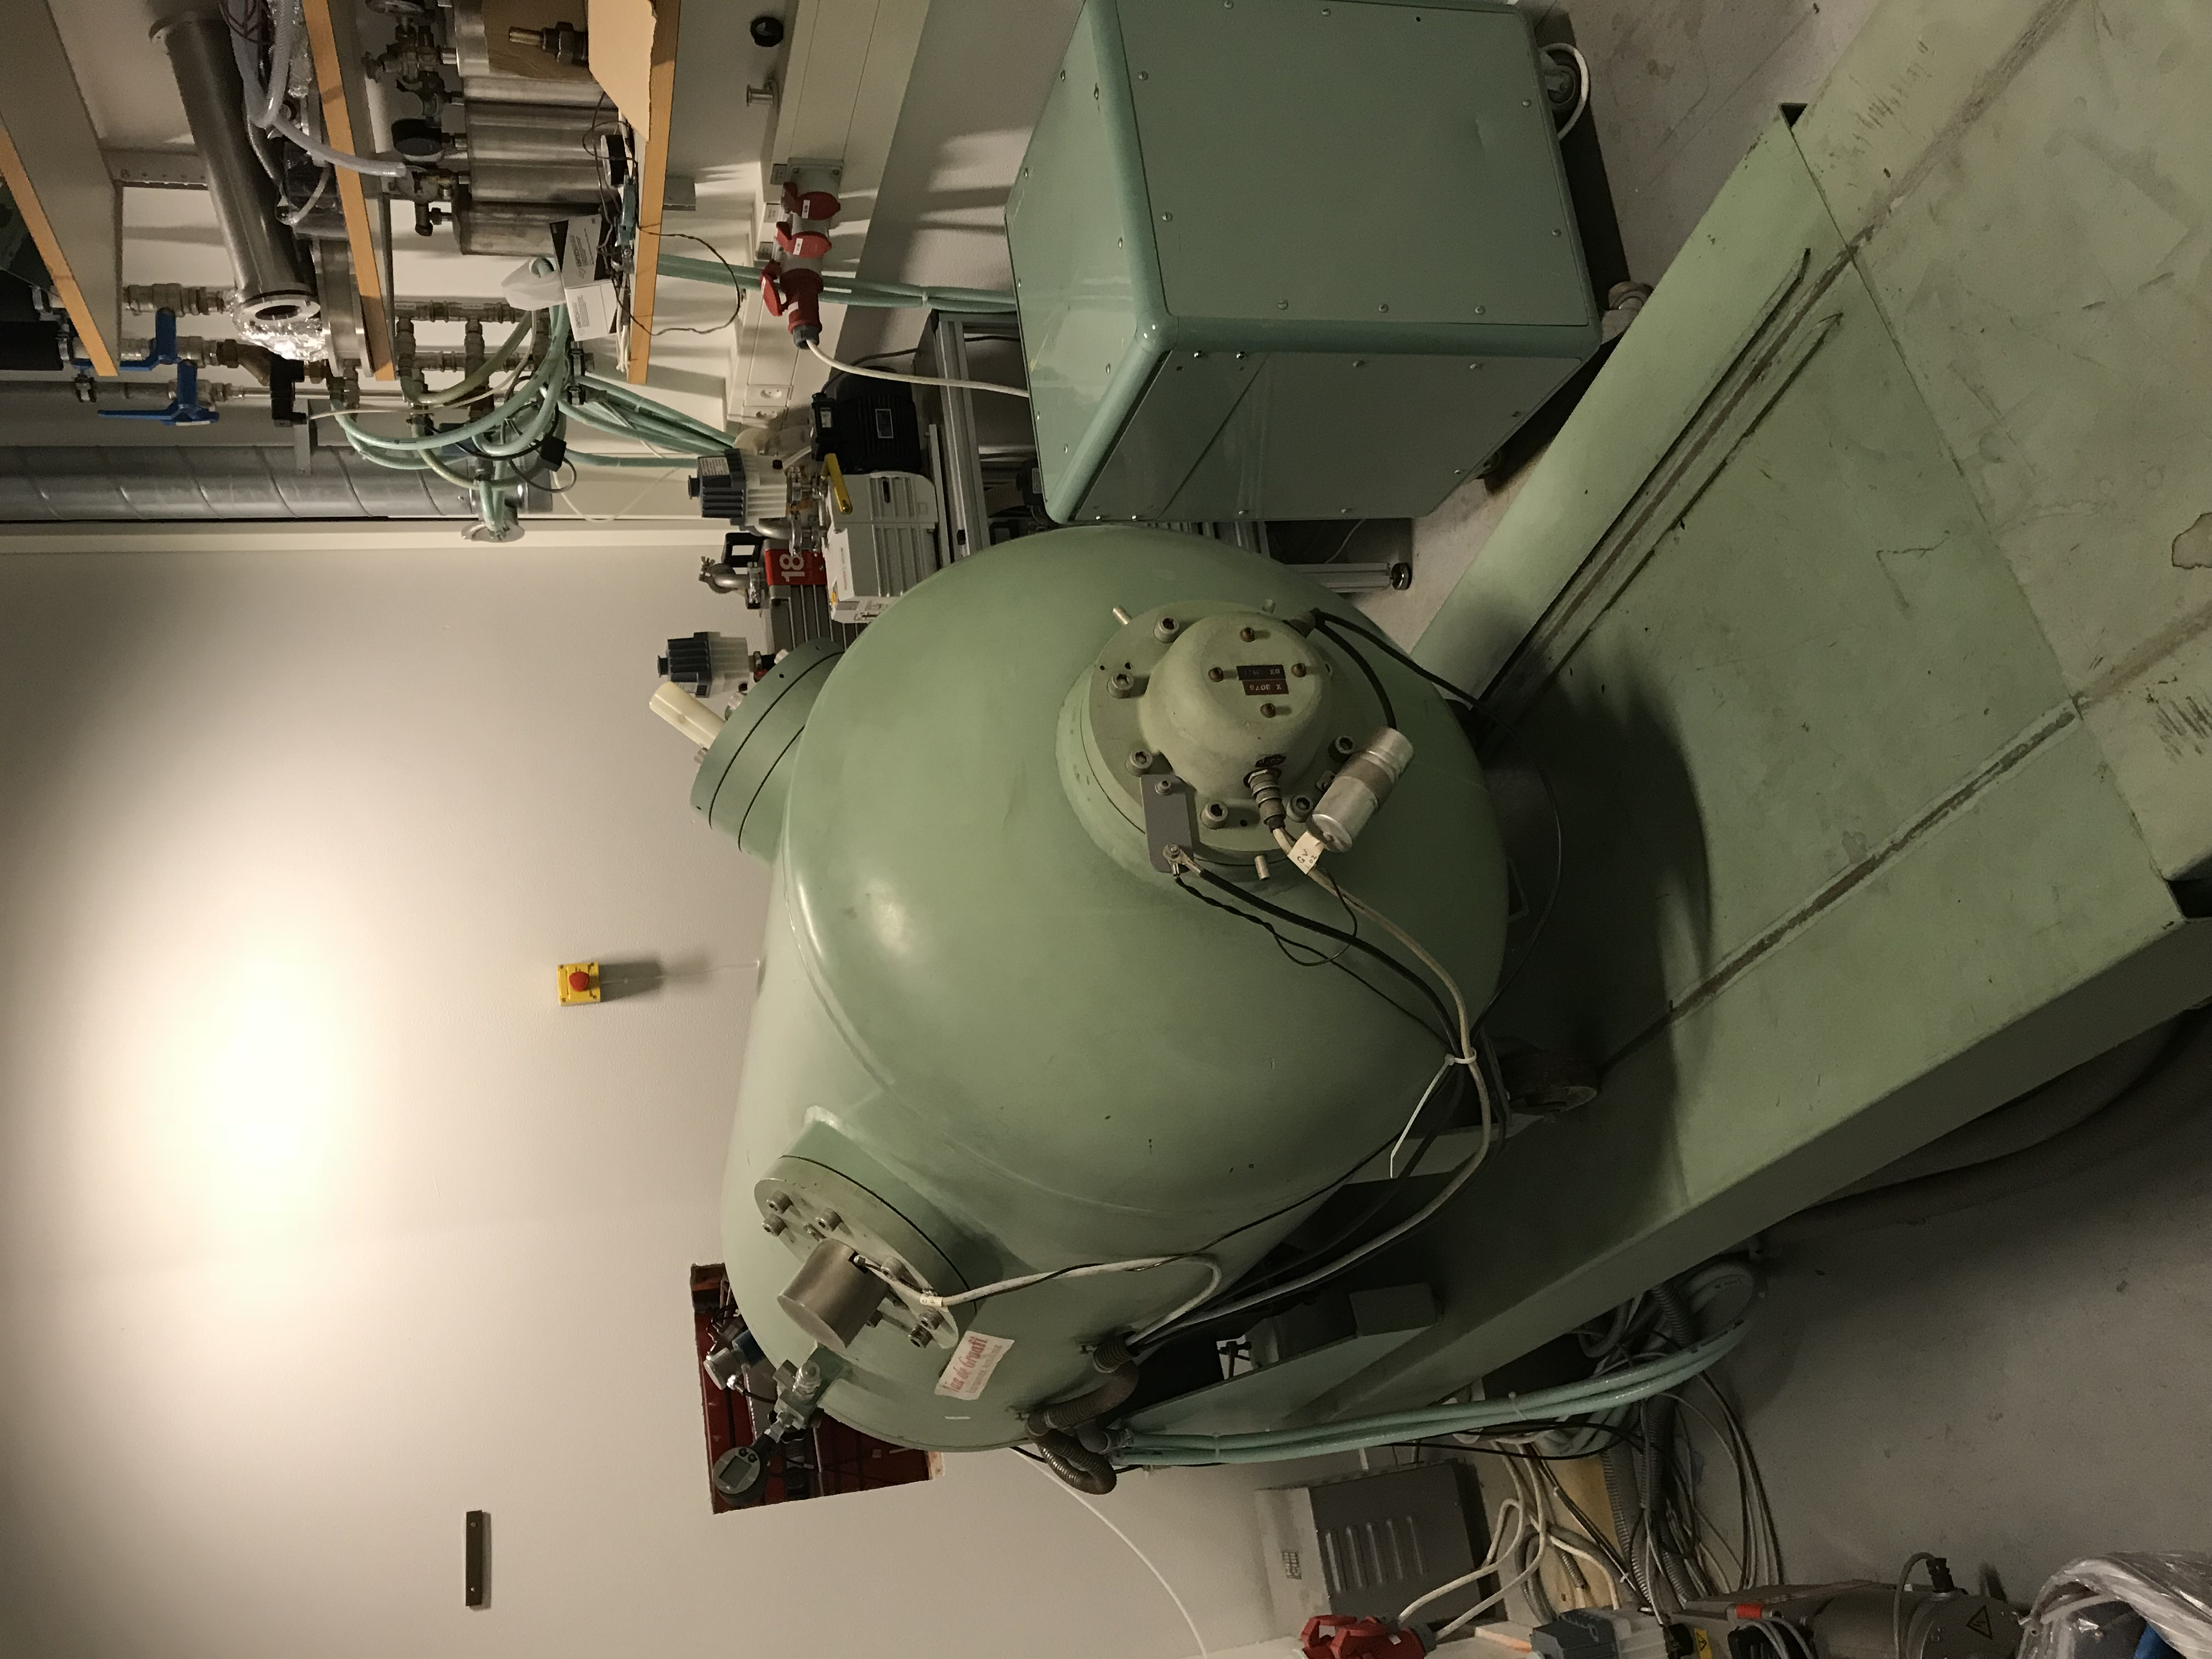
\includegraphics[angle=-90, trim={35cm, 0cm, 27cm, 0cm}, clip,  width=0.99\columnwidth]{setup3}
    \caption{The Van-de-Graaf accelerator.}
    \label{fig_setup3}
\end{figure}
%
Acceleration of the ions was controllable by changing the voltage drop on the
dashboard (see \cref{fig_setup2}) and thus also the kinetic energy of the
incoming beam. This will be described further in the section Procedure.

The beamline was placed in an angle relative to the accelerator. By changing the magnetic field strength of the electromagnet, one could choose which of the two possible incoming ions were deflected into the beamline and thus directed towards scattering on the target material at the end of the beamline.
The motion of a charged particle in a magnetic field is governed by the Lorentz force law, and as the trajectory of the motion is traced as part of a circle, one obtains the necessary equality for the motion to be\footnote{Dealing with forces and spatial confinements to circular paths this is true in the classical regime. This is not the case for a full relativistic and quantum mechanical description.}
\begin{equation}
F_|m| = QvB = F_|cp| = \frac{mv^2}{r}.
\end{equation}
From this a ratio between the two magnetic fields needed for the respective ions is
\begin{align}
    R_|B| = & \frac{B(\mathrm{{H_2}^+})}{B(\mathrm{H^+})} = \frac{m(\mathrm{{H_2}^+})
    v(\mathrm{{H_2}^+})}{m(\mathrm{H^+})v(\mathrm{H^+})}\\
    & 2 \frac{v(\mathrm{{H_2}^+})}{v(\mathrm{H^+})} = \sqrt{2},
\end{align}

%
where it has been assumed that the mass of the two ions are related by $m(H^+) = 2m(\mathrm{{H_2}^+})$ and the speed of each ion is given as $v(\mathrm{X}) = \sqrt{\frac{2E}{m(\mathrm{X})}}$. 
%
Given one of the magnetic fields, the other is determined from this ratio factor. The following magnetic field strengths were used:
%
\begin{equation}
    B(\mathrm{H^+}) = \SI{1070}{\gauss} \quad B(\mathrm{{H_2}^+}) = \SI{1513}{\gauss}
\label{}
\end{equation}
%
Conclusively, by changing the magnetic field strength, one changes the
incomming ion. BE AWARE: The magnetic field can change over the time scale of meassurements
due to mechanical heating of the metal in the electromagnet. This leads to expansion and thus
the magnetic field will be reduced.
%
\begin{figure}[t]
    \centering
    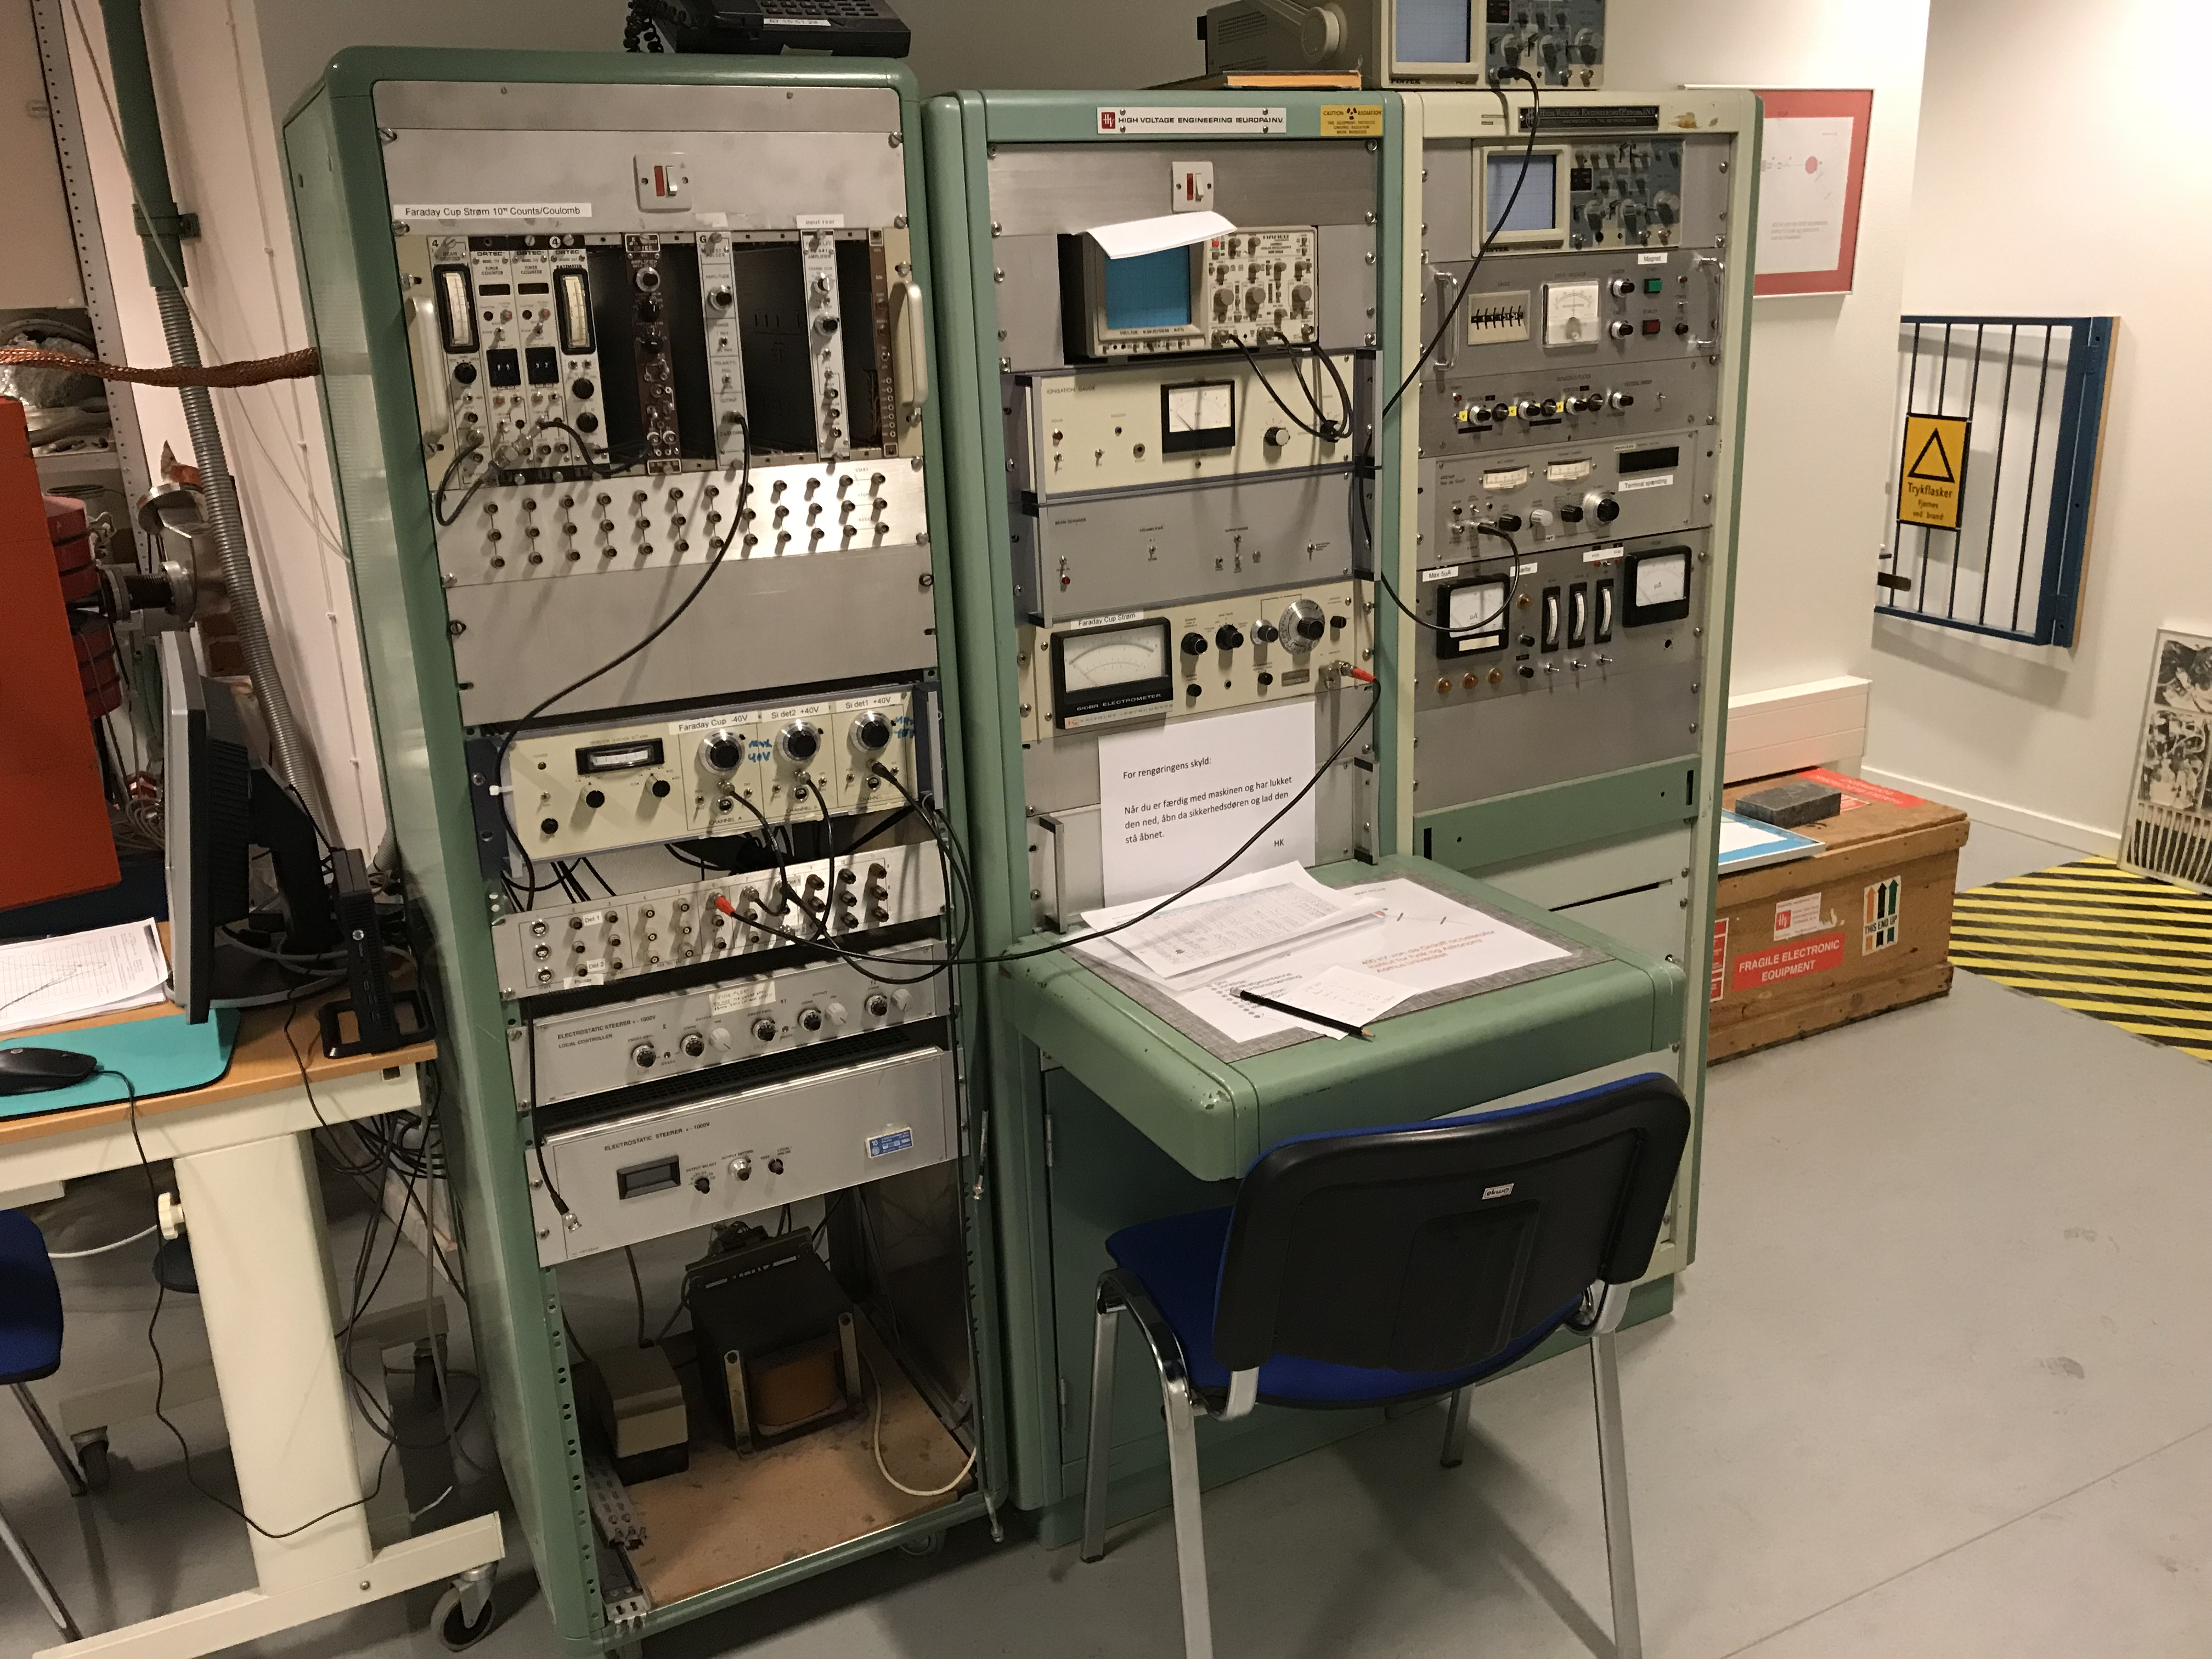
\includegraphics[width=0.99\columnwidth]{setup2}
    \caption{Overview of dashboard. Closer graphics are seen in the Procedure.}
    \label{fig_setup2}
\end{figure}
%
\begin{figure}[t]
    \centering
    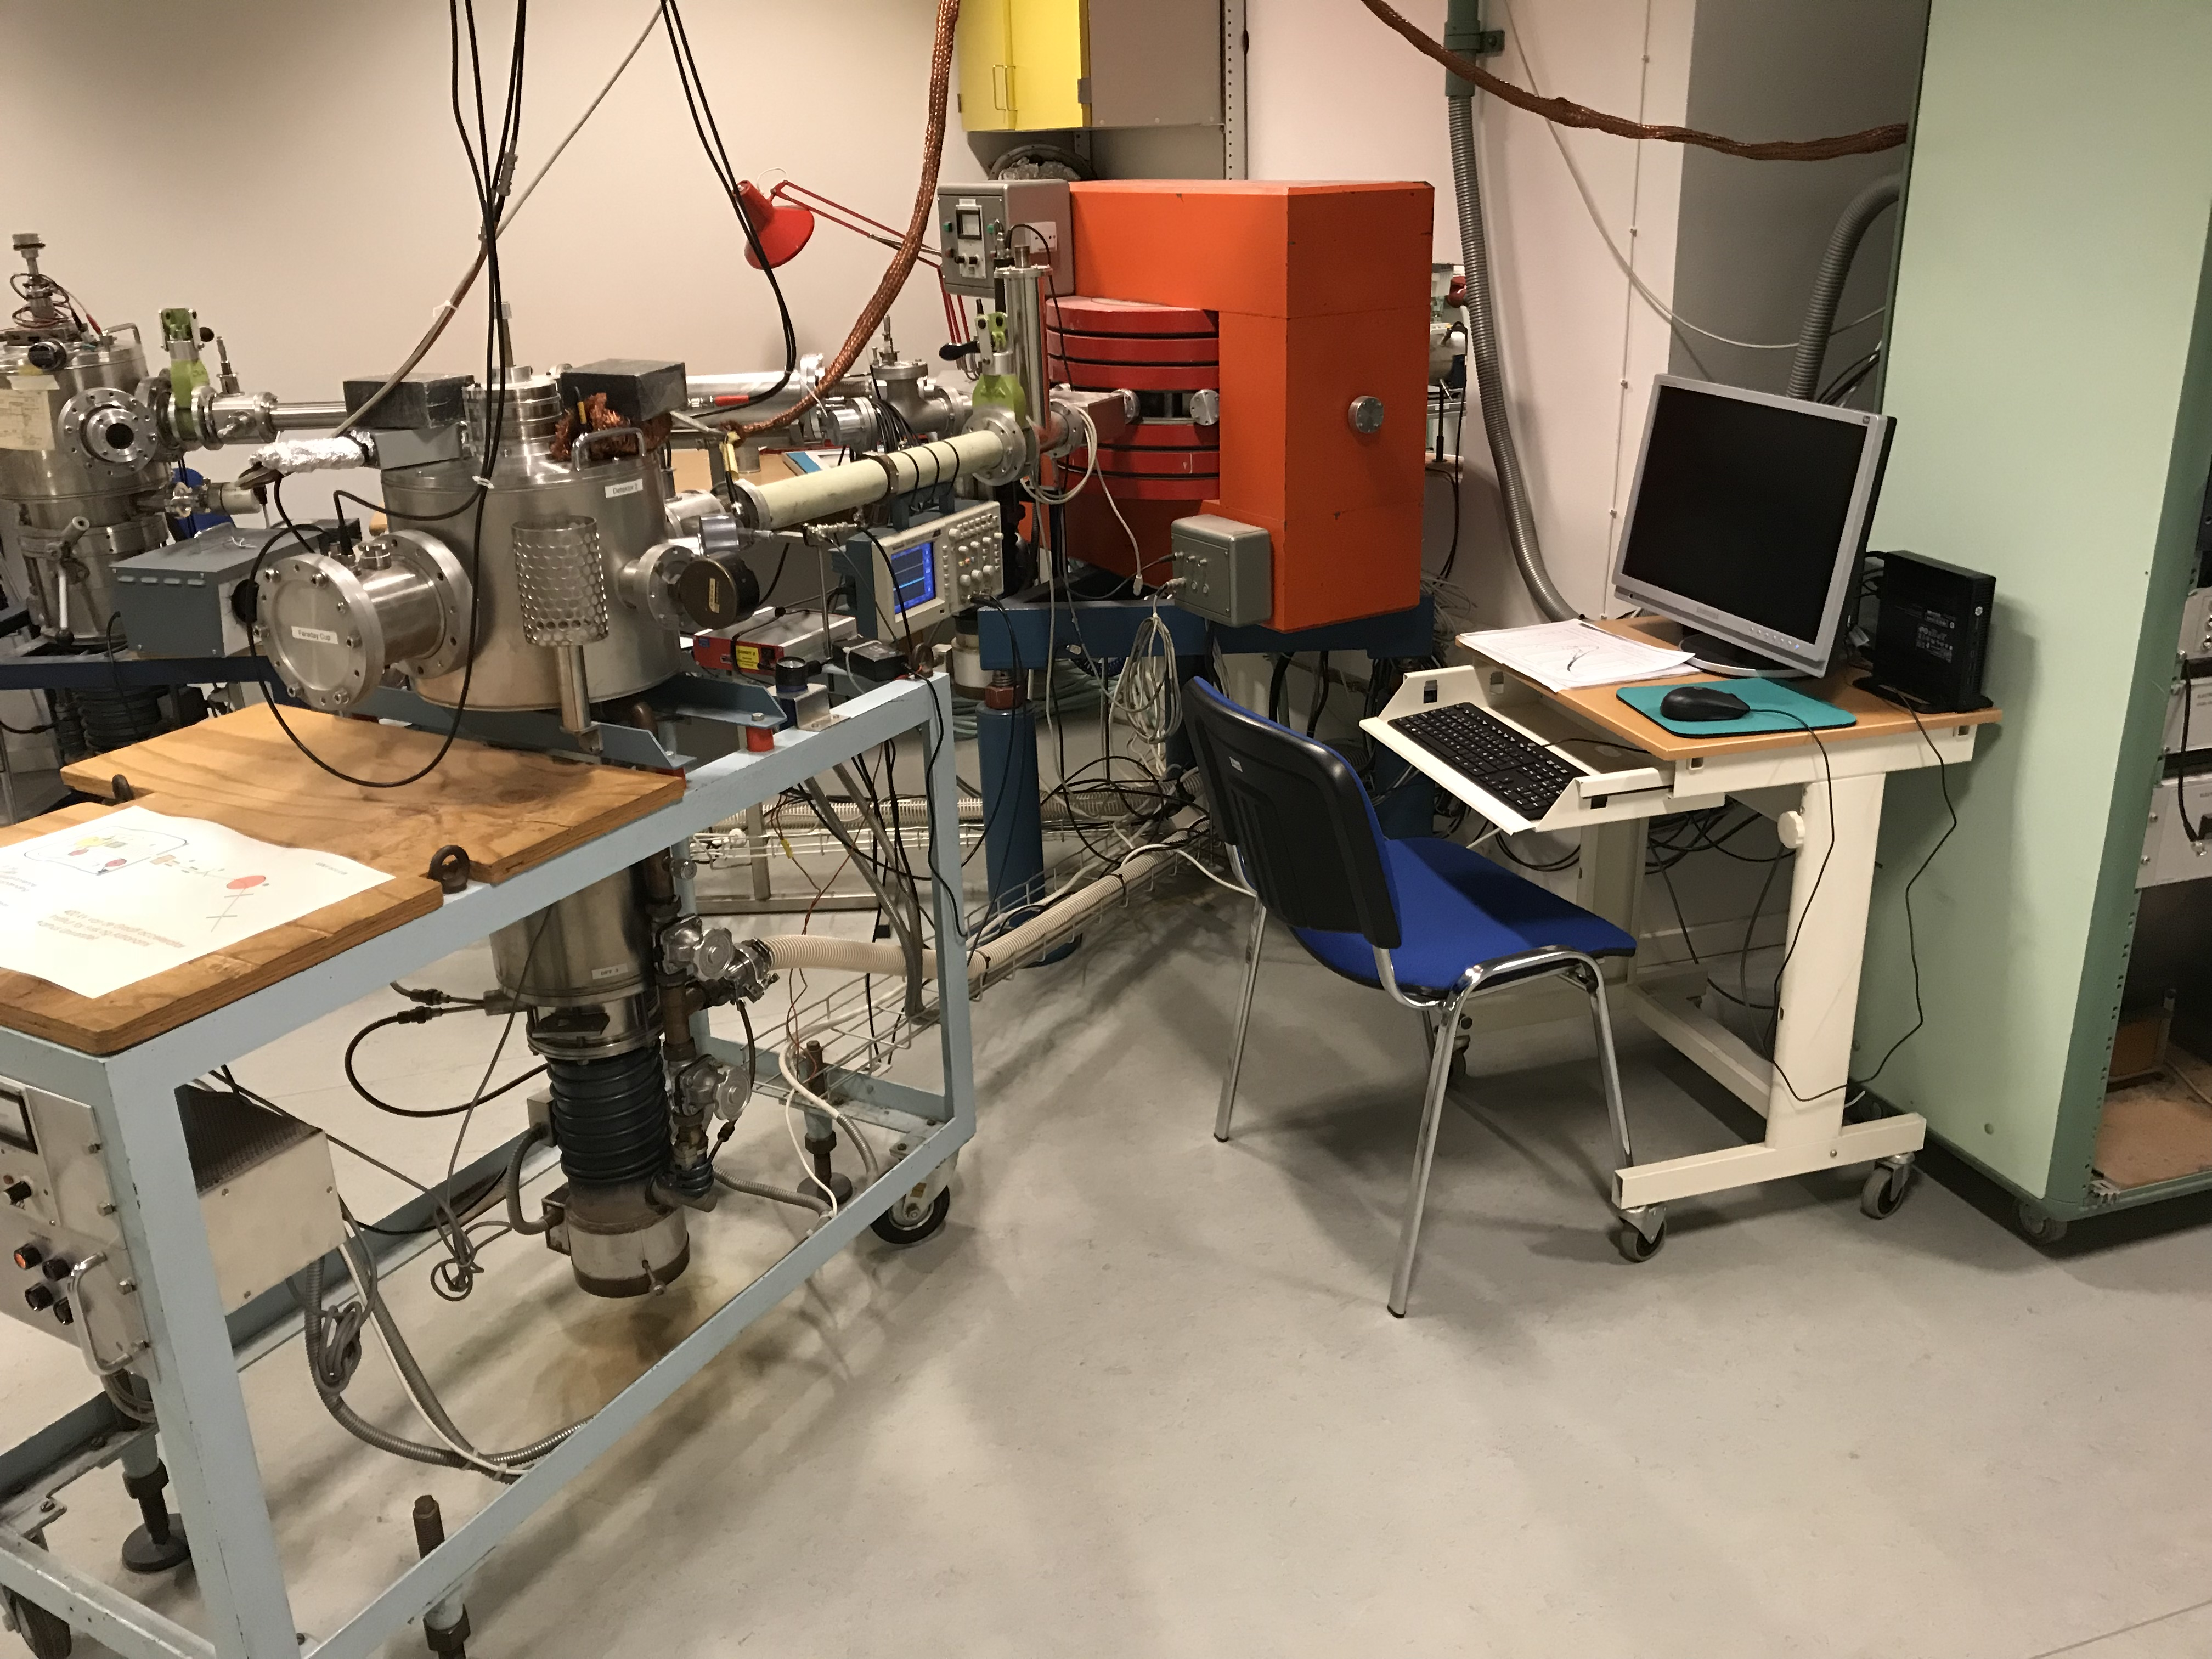
\includegraphics[width=0.99\columnwidth]{setup1}
    \caption{Overview of detector and electromagnet (red brick).}
    \label{fig_setup1}
\end{figure}
%
\begin{figure}[t]
    \centering
    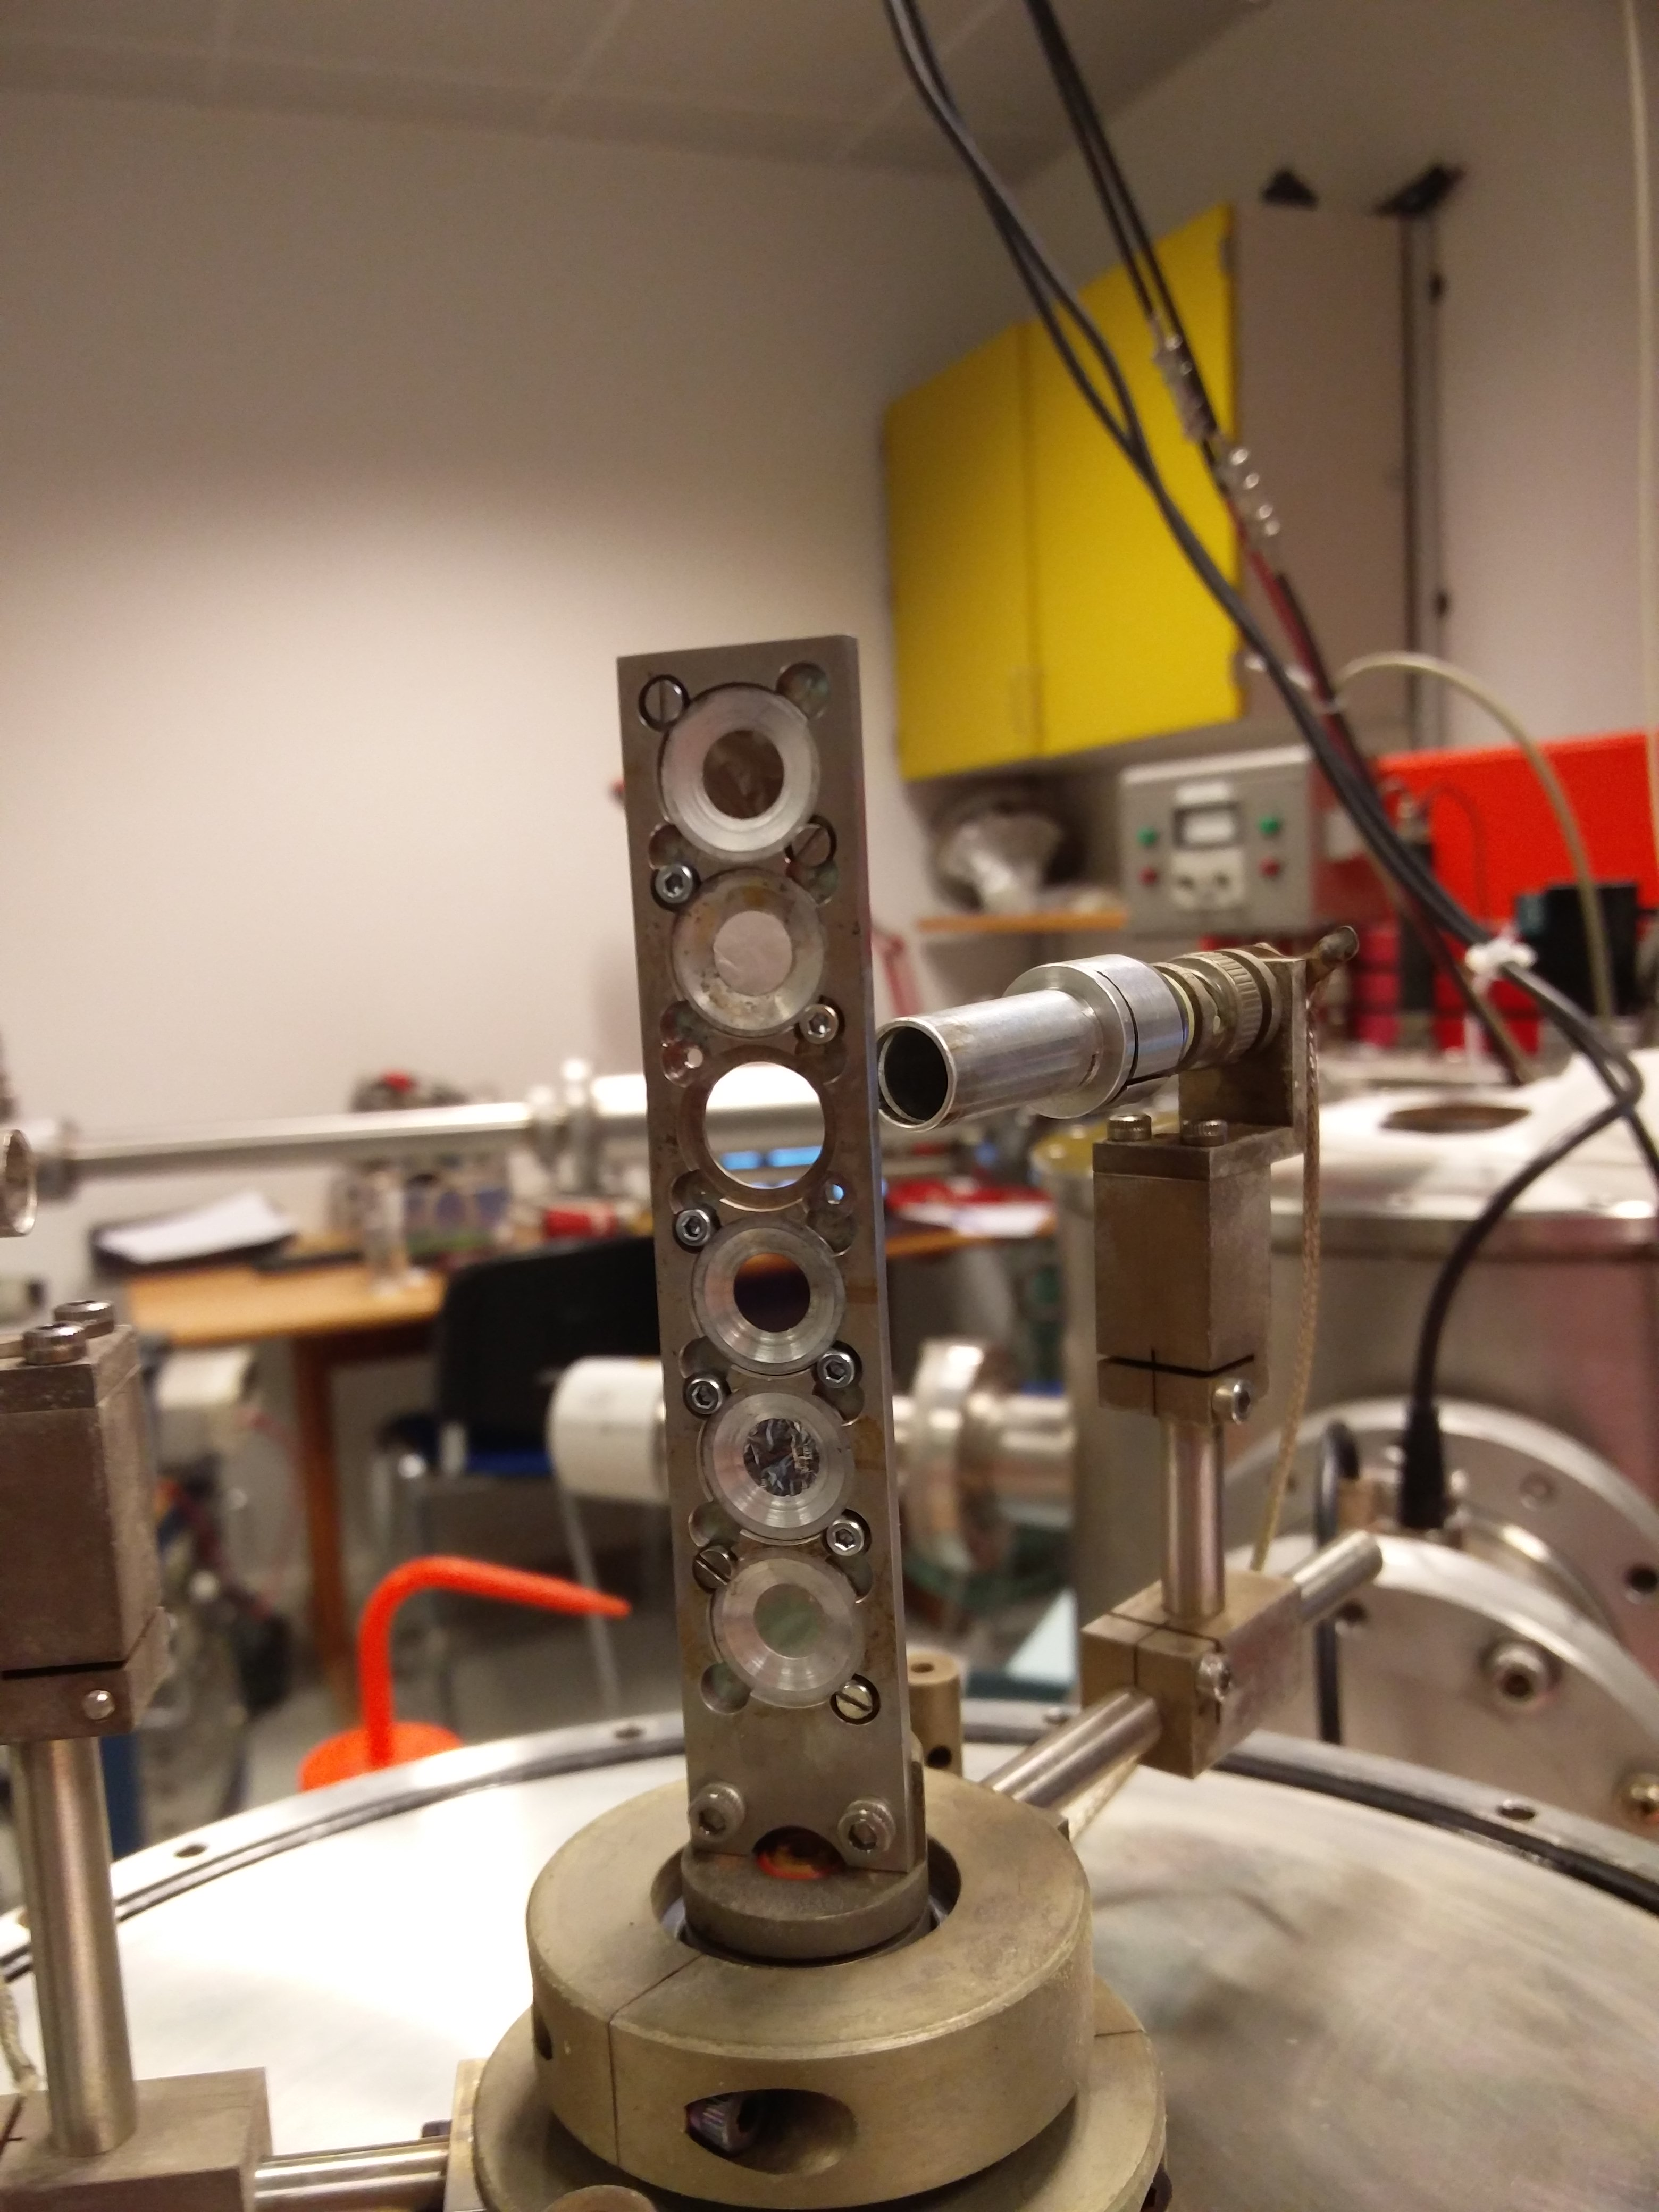
\includegraphics[trim={0cm, 10cm, 0cm, 40cm}, clip, width=0.99\columnwidth]{setup4}
    \caption{The equipment had a failure, so the targets were changed. We were
    lucky to get this picture of both detector and targets.}
    \label{fig_setup4}
\end{figure}
%
From the beamline the particles were directed toward a chosen target material
(see \cref{fig_setup4}), where they were scattered on atomic nuclei of the
target. A detector was placed at a movable position around the target, such
that scattering angles up $160$ degrees could be measured.

The detector was coupled to a digitizer connected to a computer. During
measurements the digitizer started a clock inside it. When the detector was hit
by a particle, the digitizer translated the measured energy into a digital
number and sent the number and the corresponding time stamp to the computer.
The program Mc2Analyzer was used to handle the data. The digital number is an
arbitrary number called a channel number. It is translatable to the actual
energy by a linear factor plus an offset. In order to convert these channel
numbers to correct energies of the scattered particles a calibration was done.

\subsection{Calibration}
An energy meassurement of the scattered ion gives a digitial output, which we call
a channel number (or bin number). These hold no physical interpretation, but
can be translated to the equivalent energy of the scattered particle. To
convert these channel numbers, a calibration is necesarry. 

Assuming a linear relationship between the energy and the channel number the
energy can be found as
\begin{equation}
E = \alpha(k - k_0),
\end{equation}
where $k$ is the meassured channel and $k_0$ and $\alpha$ are parameters. The
parameters in the relation is determined by a two step program.

\subsubsection{Determing Zero-Amplitude constant}
First, by connecting a pulser (variable output voltage), a relation between the
varied energy and the corresponding channel number is obtained. 
We did this for equidistant pulsed energies, but also the lowest threshold
energy. Plotting the count numbers as a function of bin numbers, and fitting a
gaussian to each value of pulsed energy, one would obtain all parameters of the
gaussian (amplitude, mean value and standard deviation), which was used to
estimate the mean bin number, within an uncertainty of the gaussian standard deviation (see
\cref{fig_gaussian_fit}). 

Afterwards, each mean channel number was plotted as a function of the pulser
energy, and this surely shows a linear relation, which also was fitted. The
intersection is interpretated as the bin number for zero amplitude ($k_0$). A
plot can be seen on \cref{fig_linear_fit}.

%\cref{fig_gaussian_fit}  shows the count distribution as function of channels for the amplitude fitted with gaussian function. The data clearly follows a gaussian distribution and the data points are, within uncertainty, well described by a gausian distribution. 

%However, another method is used to determine the zero-amplitude constant $k_0$. Different energies are generated using a pulse generator by changing the amplitude (corresponding to a change of resistance). For each fixed amplitude, a normal distribution of counts around a certain mean channel is obtained. The mean channel (also called the centroid) is determined from a Gaussian fit to the distribution. 

\begin{figure}[h]
\centering
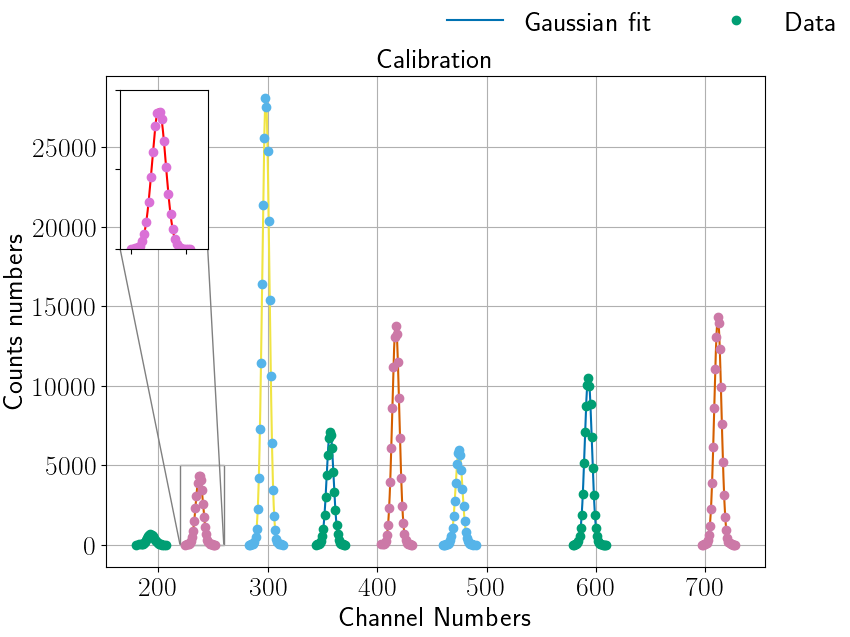
\includegraphics[width=0.99\columnwidth]{gaussian_fit}
\caption{Gaussian fit of all data values. This was used to estimate the mean
bin number (channel number), and the uncertainty of this bin number, in the
energy-calibration.}
\label{fig_gaussian_fit}
\end{figure}

\begin{figure}[h]
\centering
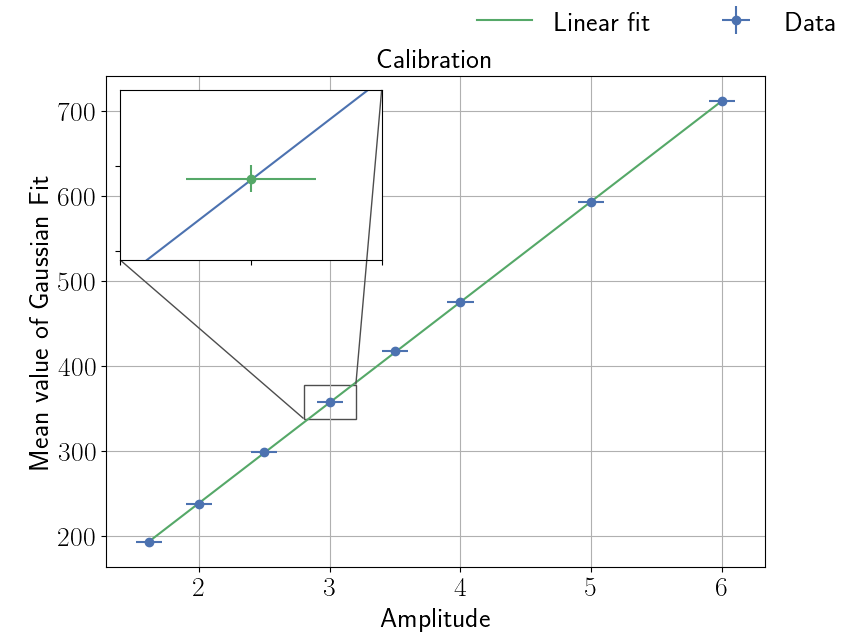
\includegraphics[width=0.99\columnwidth]{k0_plotting}
\caption{Linear fit of the mean values as a function of amplitude. This was
used to determine the zero-amplitude constant $k_0$.}
\label{fig_linear_fit}
\end{figure}

\subsection{Targets}
The targets of interest in this experiment was a thin gold coated carbon plate. The gold coating was about one tenth of the carbon thickness. The thickness of the carbon plate have previously been determined as $\SI{250}{\angstrom}$, and the thickness of the gold coating as $\SI{25}{\angstrom}$.\footnotemark \footnotetext{The estimated thickness of each target available have been determined by the previous users of the experimental setup and written down on the whiteboard next to the setup.} 
The target was placed in holder, which contains several other targets. The height of the holder was fixed, though it was not investigated whether the marked height was optimal with respect to the beam position.\\

When measuring proton scattering at different angles, the blind angles of the target holder may cause a problem. In order to avoid the targets "blind-spots", the target was turned at an angle following the detector while still avoiding the incoming proton beam to hit a blind angle. The blind angles of the holder are around $\pm 30 \si{\degree}$ in each side of the target holder, see figure .  
  
\subsubsection{Determining alpha}
As described in the previous section, the magnetic field strength of the
electromagnet can be adjusted to deflect either $\mathrm{H^+}$ or
$\mathrm{{H_2}^+}$ into the beamline. For each of these a data point of energy
related to channel number can be found.
By considering energy and momentum conservation for elastic scattering in two
dimensions the energy of the scattered particles $E_f$ can be found from the
incident proton energy and the scattering angle as:
\begin{equation}
E_f = \left( \frac{m_|p| \cos\theta + \sqrt{{m_|t|}^2 - {m_|p|}^2
\sin^2\theta}}{m_|p|+m_|t|} \right)^2 E_|i|,
\label{eq_5}
\end{equation}
where $E_|i|$ is the energy of the incident beam particles, $m_|p|$ and $m_|t|$ are
the masses of the incident protons and the target particles, respectively, and
$\theta$ is the angle between the direct outgoing non-scattered beam and the
scattered particles - also called the scattering angle.

Unfortunately, this only give two data points one from $\mathrm{H^+}$ and
another from $\mathrm{{H_2}^+}$. Nonetheless, the incline from the linear fit
to these data points is still useful.

\begin{figure}[t]
\centering
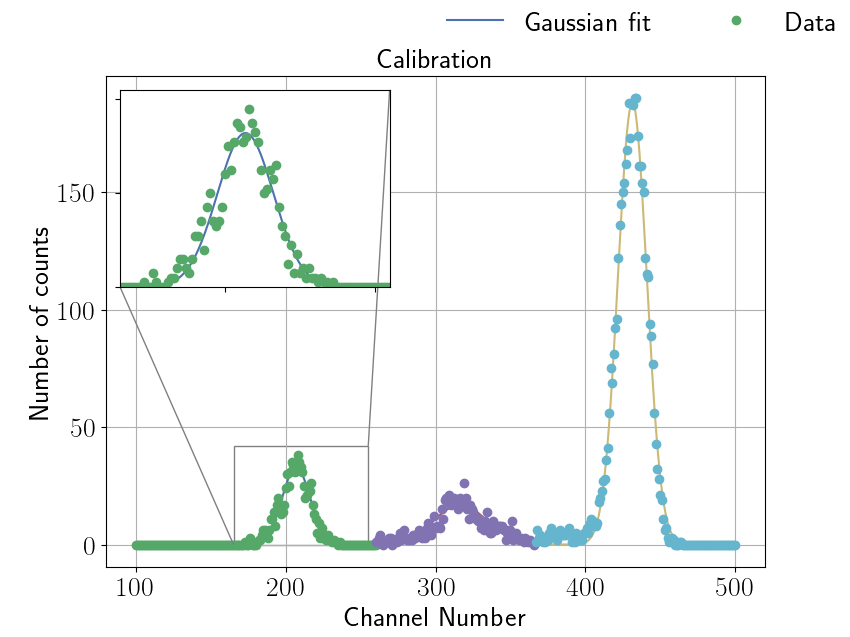
\includegraphics[width=0.99\columnwidth]{gaussian_fit2}
\caption{Gaussian fit of all data values. This was used to estimate the mean
bin number (channel number), and the uncertainty of this bin number, in the
energy-calibration.}
\label{fig_gaussian_fit2}
\end{figure}

\begin{figure}[t]
\centering
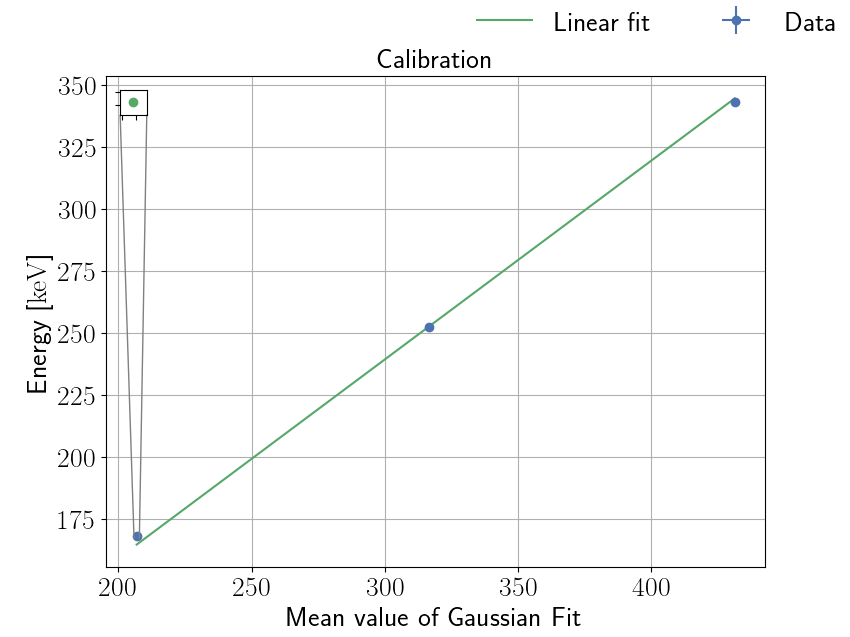
\includegraphics[width=0.99\columnwidth]{alpha_plotting}
\caption{Linear fit of the mean values as a function of amplitude. This was
used to determine the zero-amplitude constant $k_0$.}
\label{fig_linear_fit2}
\end{figure}




%TABLE WITH CORRESPONDING VALUES OF AMPLITUDE AND MEAN CHANNEL (AND THEIR UNCERTAINTIES)!
%
%FIGURE WITH AN EXAMPLE OF A GAUSSIAN FIT.

%From the fit the coefficient $k_0$ is .... 
%
%
%
%\subsection{Targets}
%Something about the different targets... Rettes til når vi ved noget mere.
%
%The targets and their corresponding thickness and areal density are noted in Table ...
%
%%\begin{table}[h]
%%\centering
%%\caption{\sl De maalte data for kalibreringen af....}
%%\begin{tabular}{l D{.}{,}{5.0} *{2}{ D{.}{,}{10.0} @{$\pm$} D{.}{,}{2.0} } %D{.}{,}{3.0}}
%%\toprule
%% \multicolumn{1}{c}{Target} & \multicolumn{2}{c}{Thickness (Å)} & %\multicolumn{2}{c}{Area density} \\
%%\midrule
%%LiF/C  &  ?  &  ? & 0.5 \\
%%B/C  &  ?  &  ?  \\
%%AL  &  ?  &  ?  \\
%%Au/C  &  ?  &  ?  \\
%%\bottomrule
%%\end{tabular}
%%\label{tbl:eksempel}
%%\end{table}

%\subsection{Scattering on atomic nuclei}
%The aim of this experiment was to use a particle accelerator to test certain dependencies of Rutherford scattering. Numerically, the Rutherford scattering differential cross section per target atom for any target atom is
%\begin{equation}
%\frac{d\sigma}{d\Omega} = 1.296 \left( \frac{Z_1 Z_2}{E_\infty [MeV] \, \sin^2 \left(\frac{\theta}{2} \right) }\right)^2\left[\frac{mb}{sr}\right],
%\end{equation}
%where $\theta$ is the scattering angle, $Z_1$  is the atomic number of the incident particles, $Z_2$ is the atomic number of the target nuclei, and $E_{\infty}$ is their kinetic energy HUSK CITE!%cite 
%. 
%In order to test these dependencies a relation between the cross section and the count rate (number of scattered particles per time) is found as
%\begin{equation}
%dN = N \, n_{\text{tar}} \, dx \,d\Omega \, \frac{d\sigma(\theta,\phi)}{d\Omega},
%\end{equation}
%where $N$ is the number of incoming particles per time, $n_\text{tar}$ is the particle density of the target, $dx$ is the thickness of the target, and $d\Omega$ is the solid angle of the detector.
%

\clearpage
\subsection{Procedure}
First thing, the Van-de-Graaf. To accelerate the beam of incomming particles,
one has to generate a hugh potential. Turning on the Belt, one hears the
mechanical rhumming. This will generate a potential difference as described
further in \cite[p.xx]{krane}.
\begin{figure}[h]
\centering
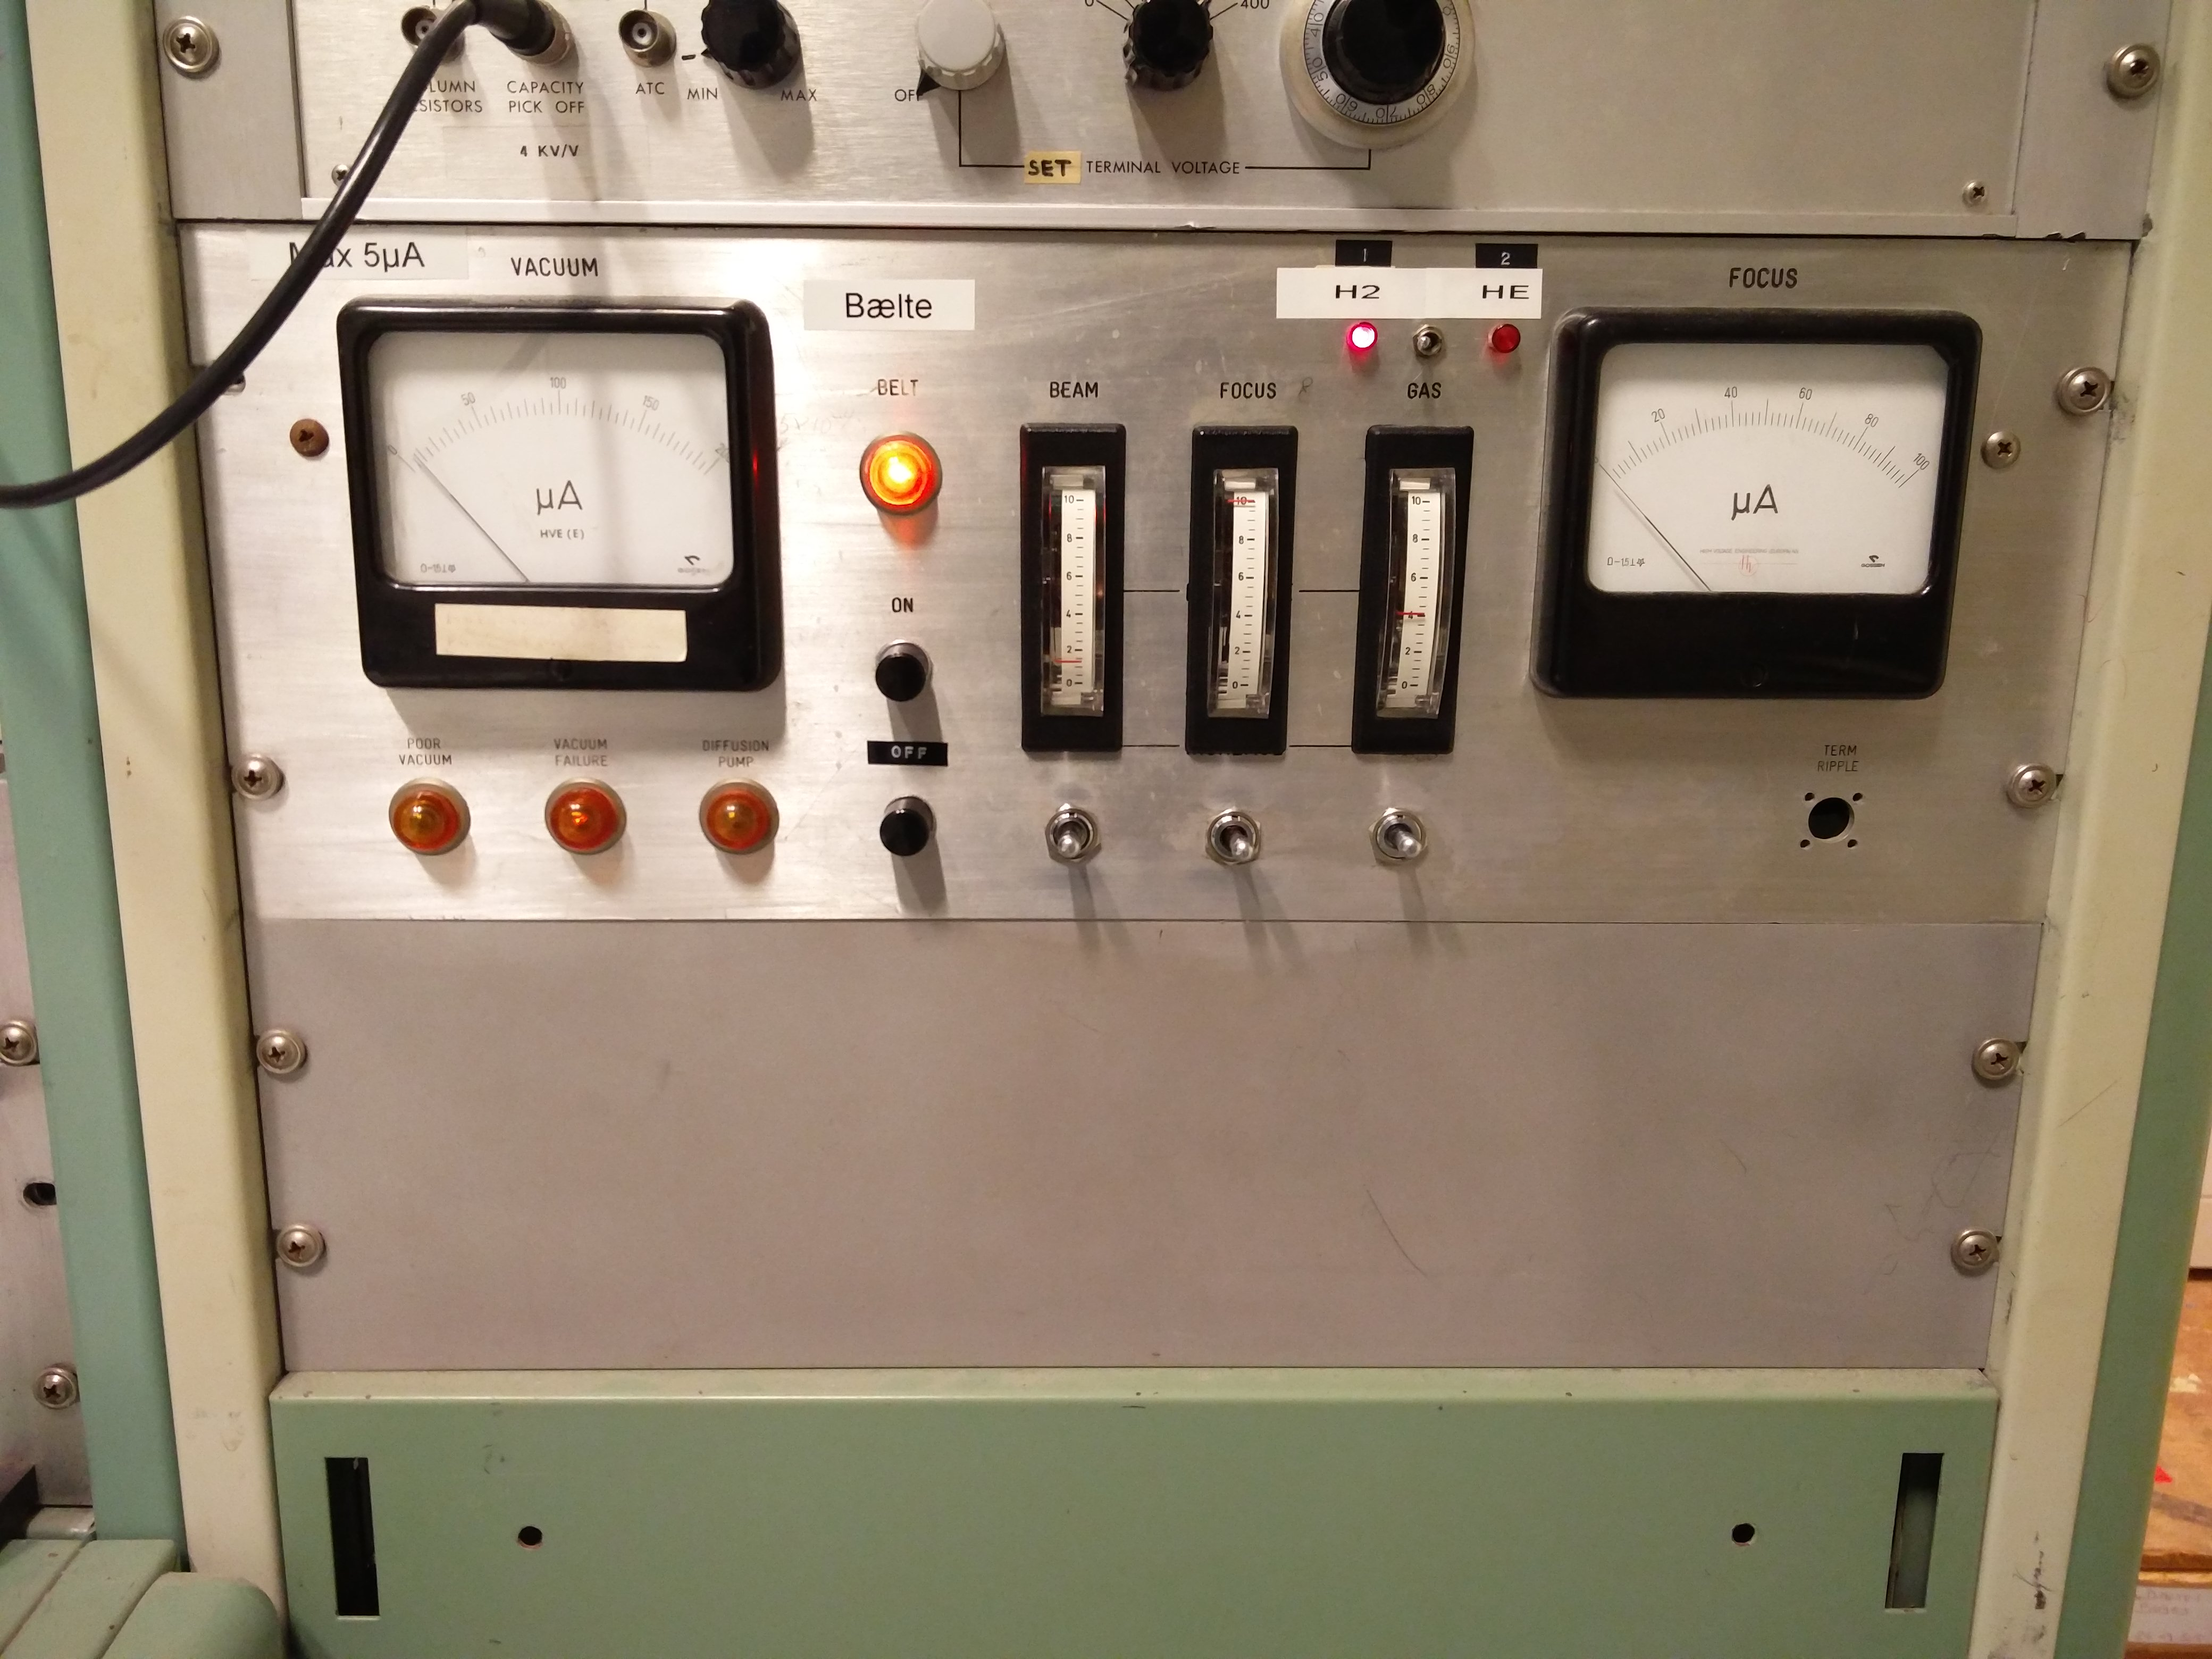
\includegraphics[trim={0, 45cm, 0, 15cm}, clip, width=0.99\columnwidth]{process1}
\caption{The belt}
\label{fig_process1}
\end{figure}

Now adjust the terminal voltage patiently towards to wanted energy. Our lab
instructor advised us to wait for each step, before going to the next.
\begin{figure}[h]
\centering
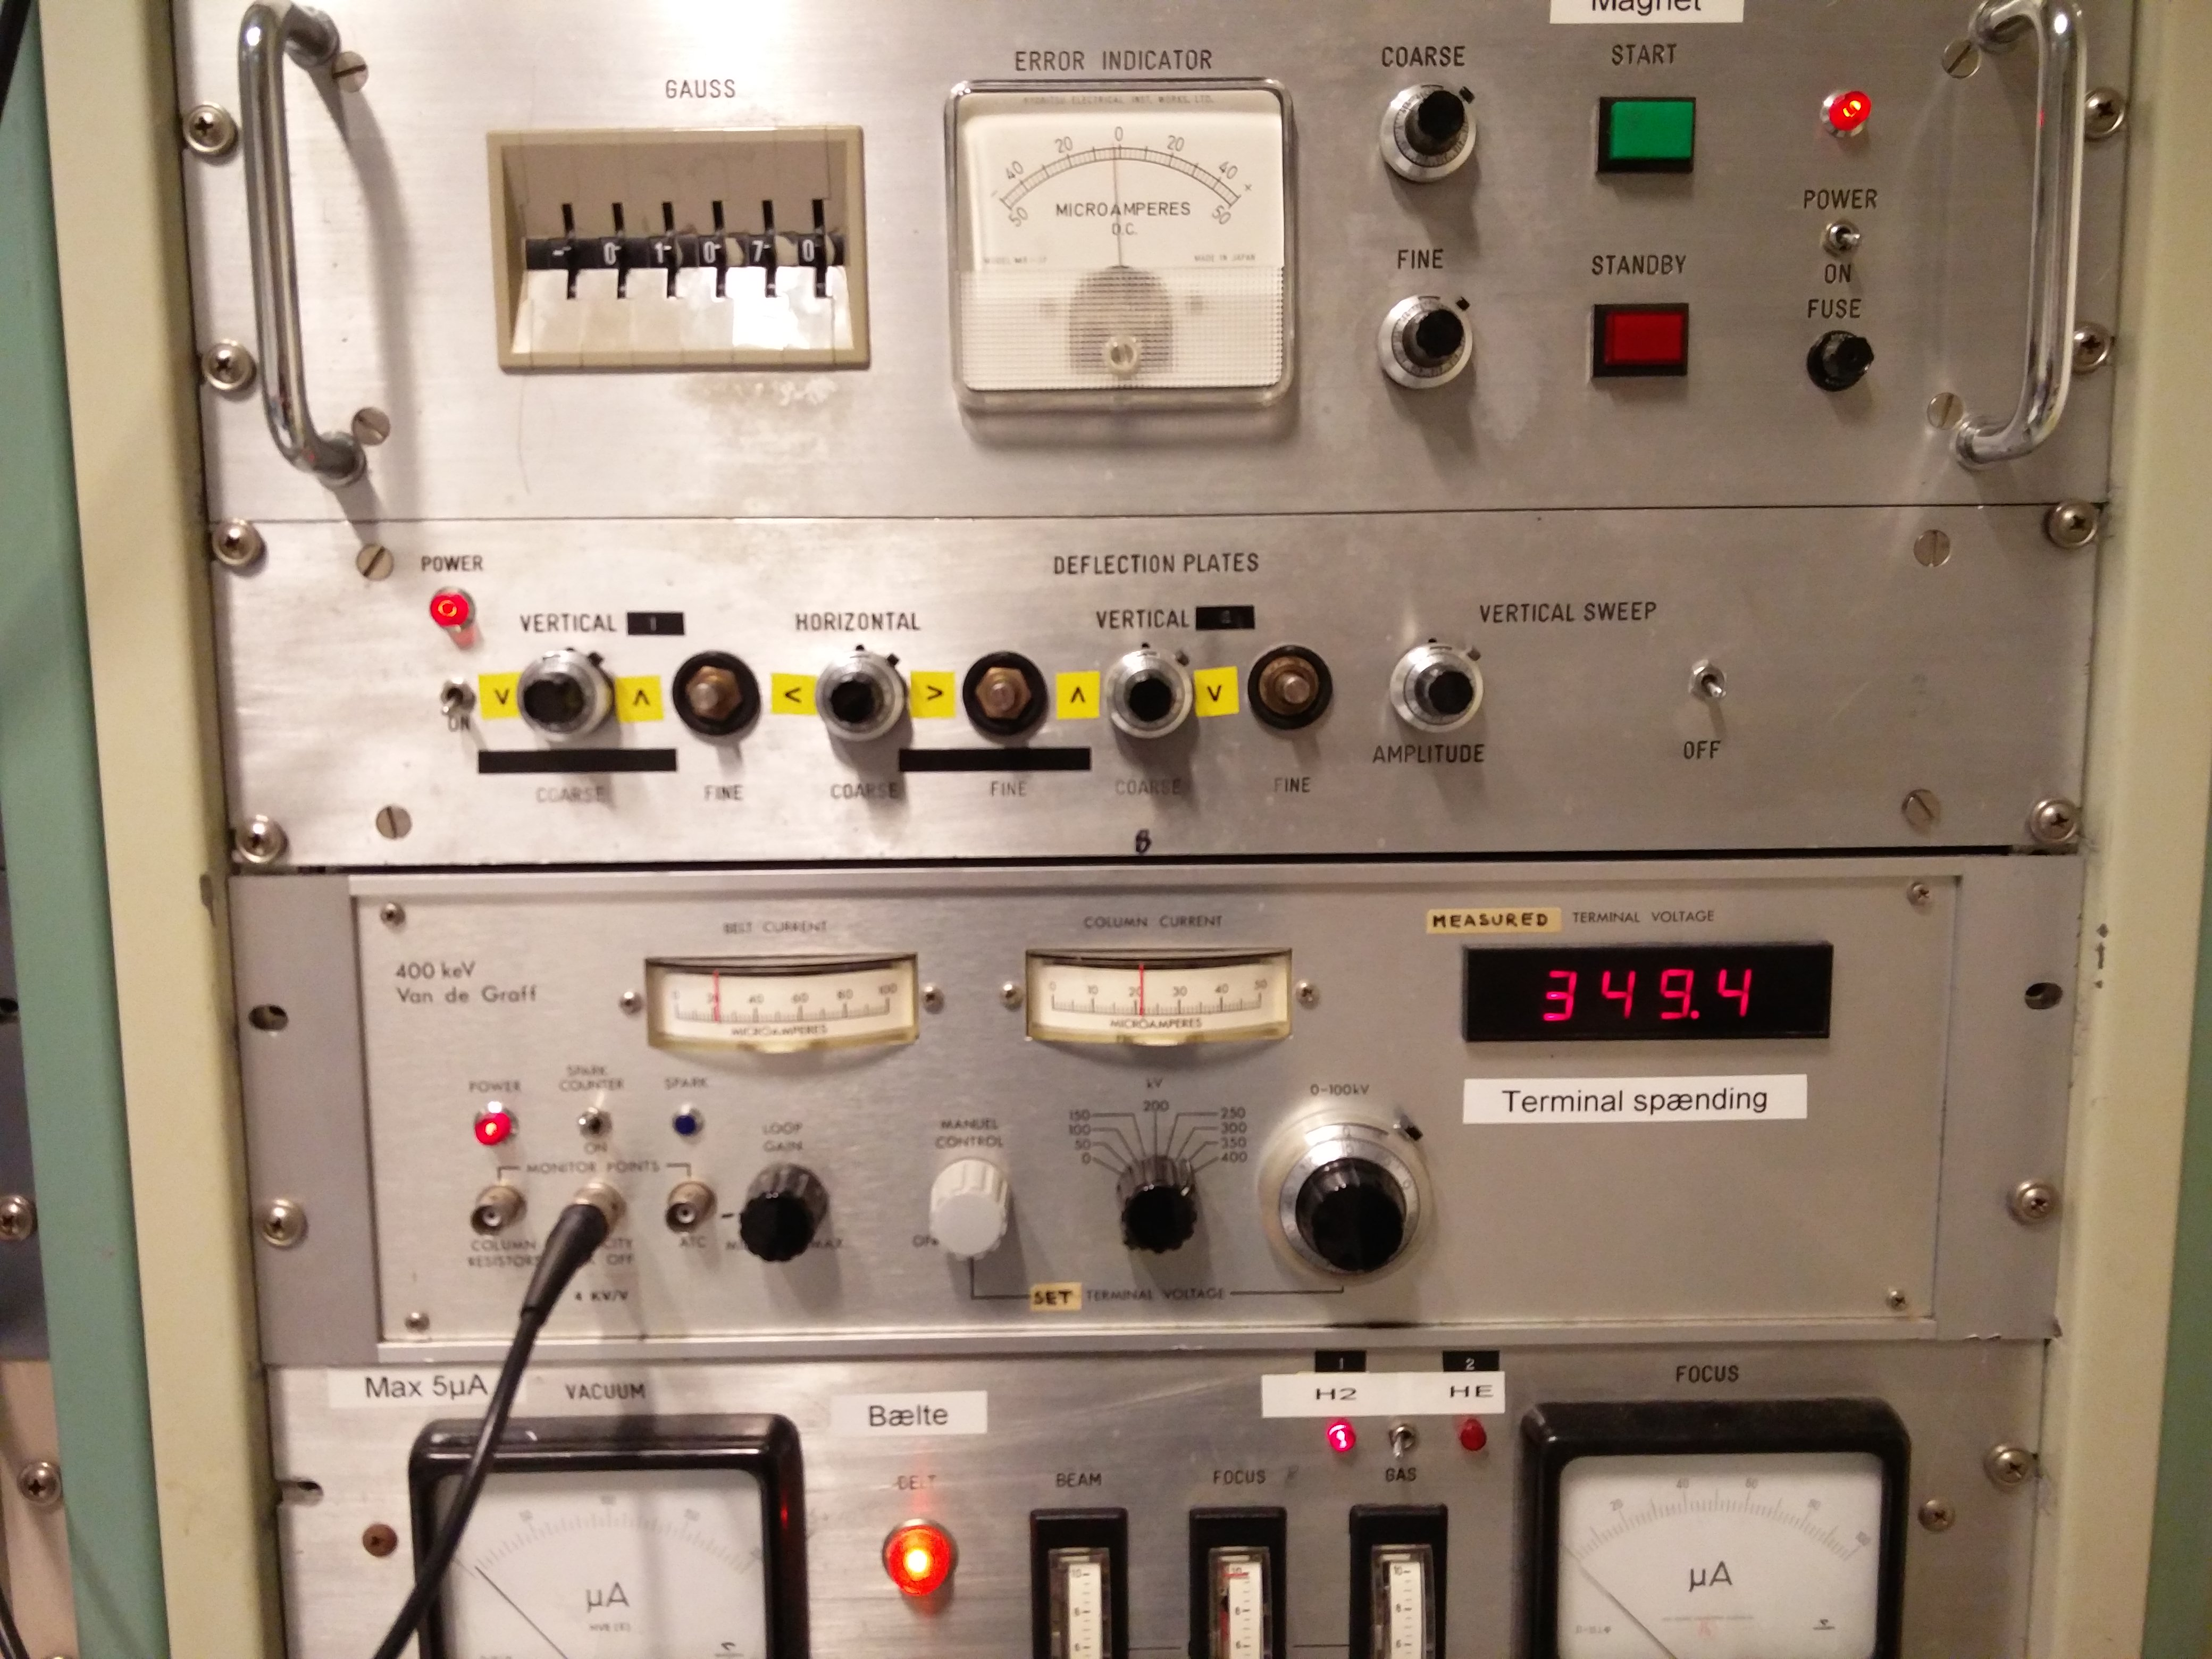
\includegraphics[trim={0, 20cm, 0, 55cm}, clip, width=0.99\columnwidth]{process2}
\caption{terminal voltage}
\label{fig_process2}
\end{figure}

Turn on the electromagnet. Remember to calculate the wanted B-field for given
element. Look on Faraday cup for received current of particles. Maximize with
fine grid (small adjustments).
\begin{figure}[h]
\centering
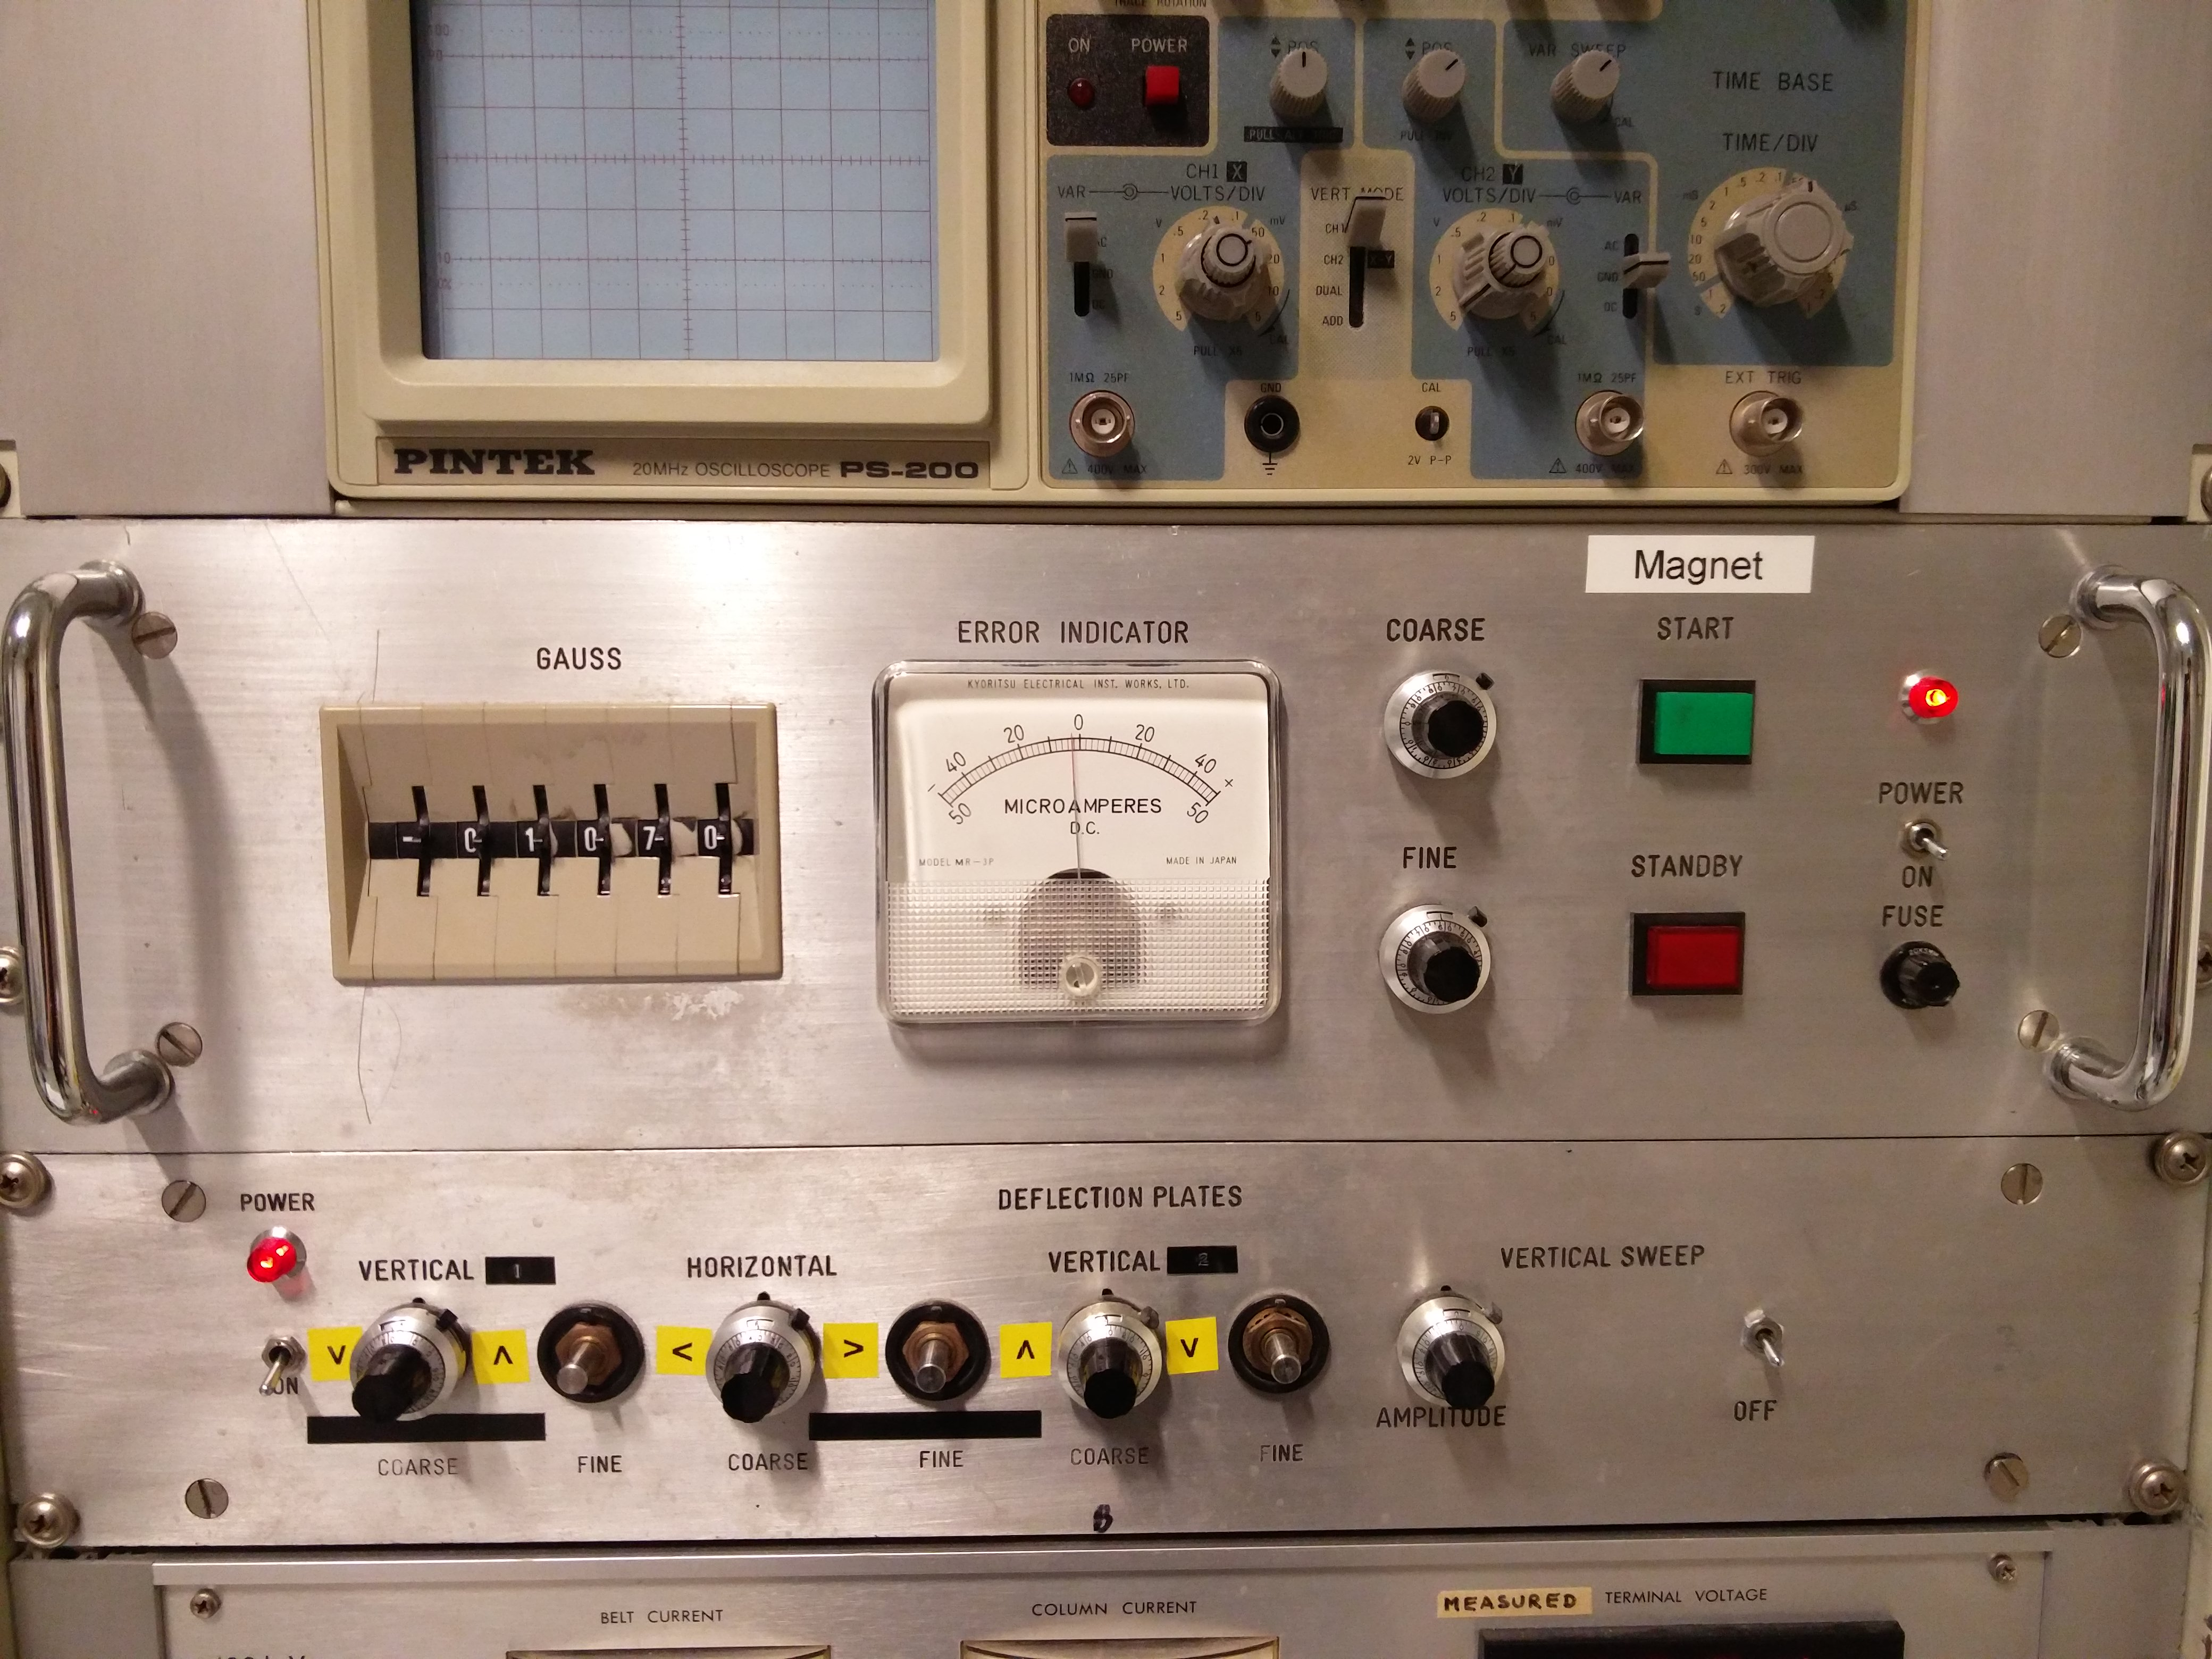
\includegraphics[trim={0, 30cm, 0, 30cm}, clip, width=0.99\columnwidth]{process3}
\caption{terminal voltage}
\label{fig_process3}
\end{figure}

\begin{figure}[h]
\centering
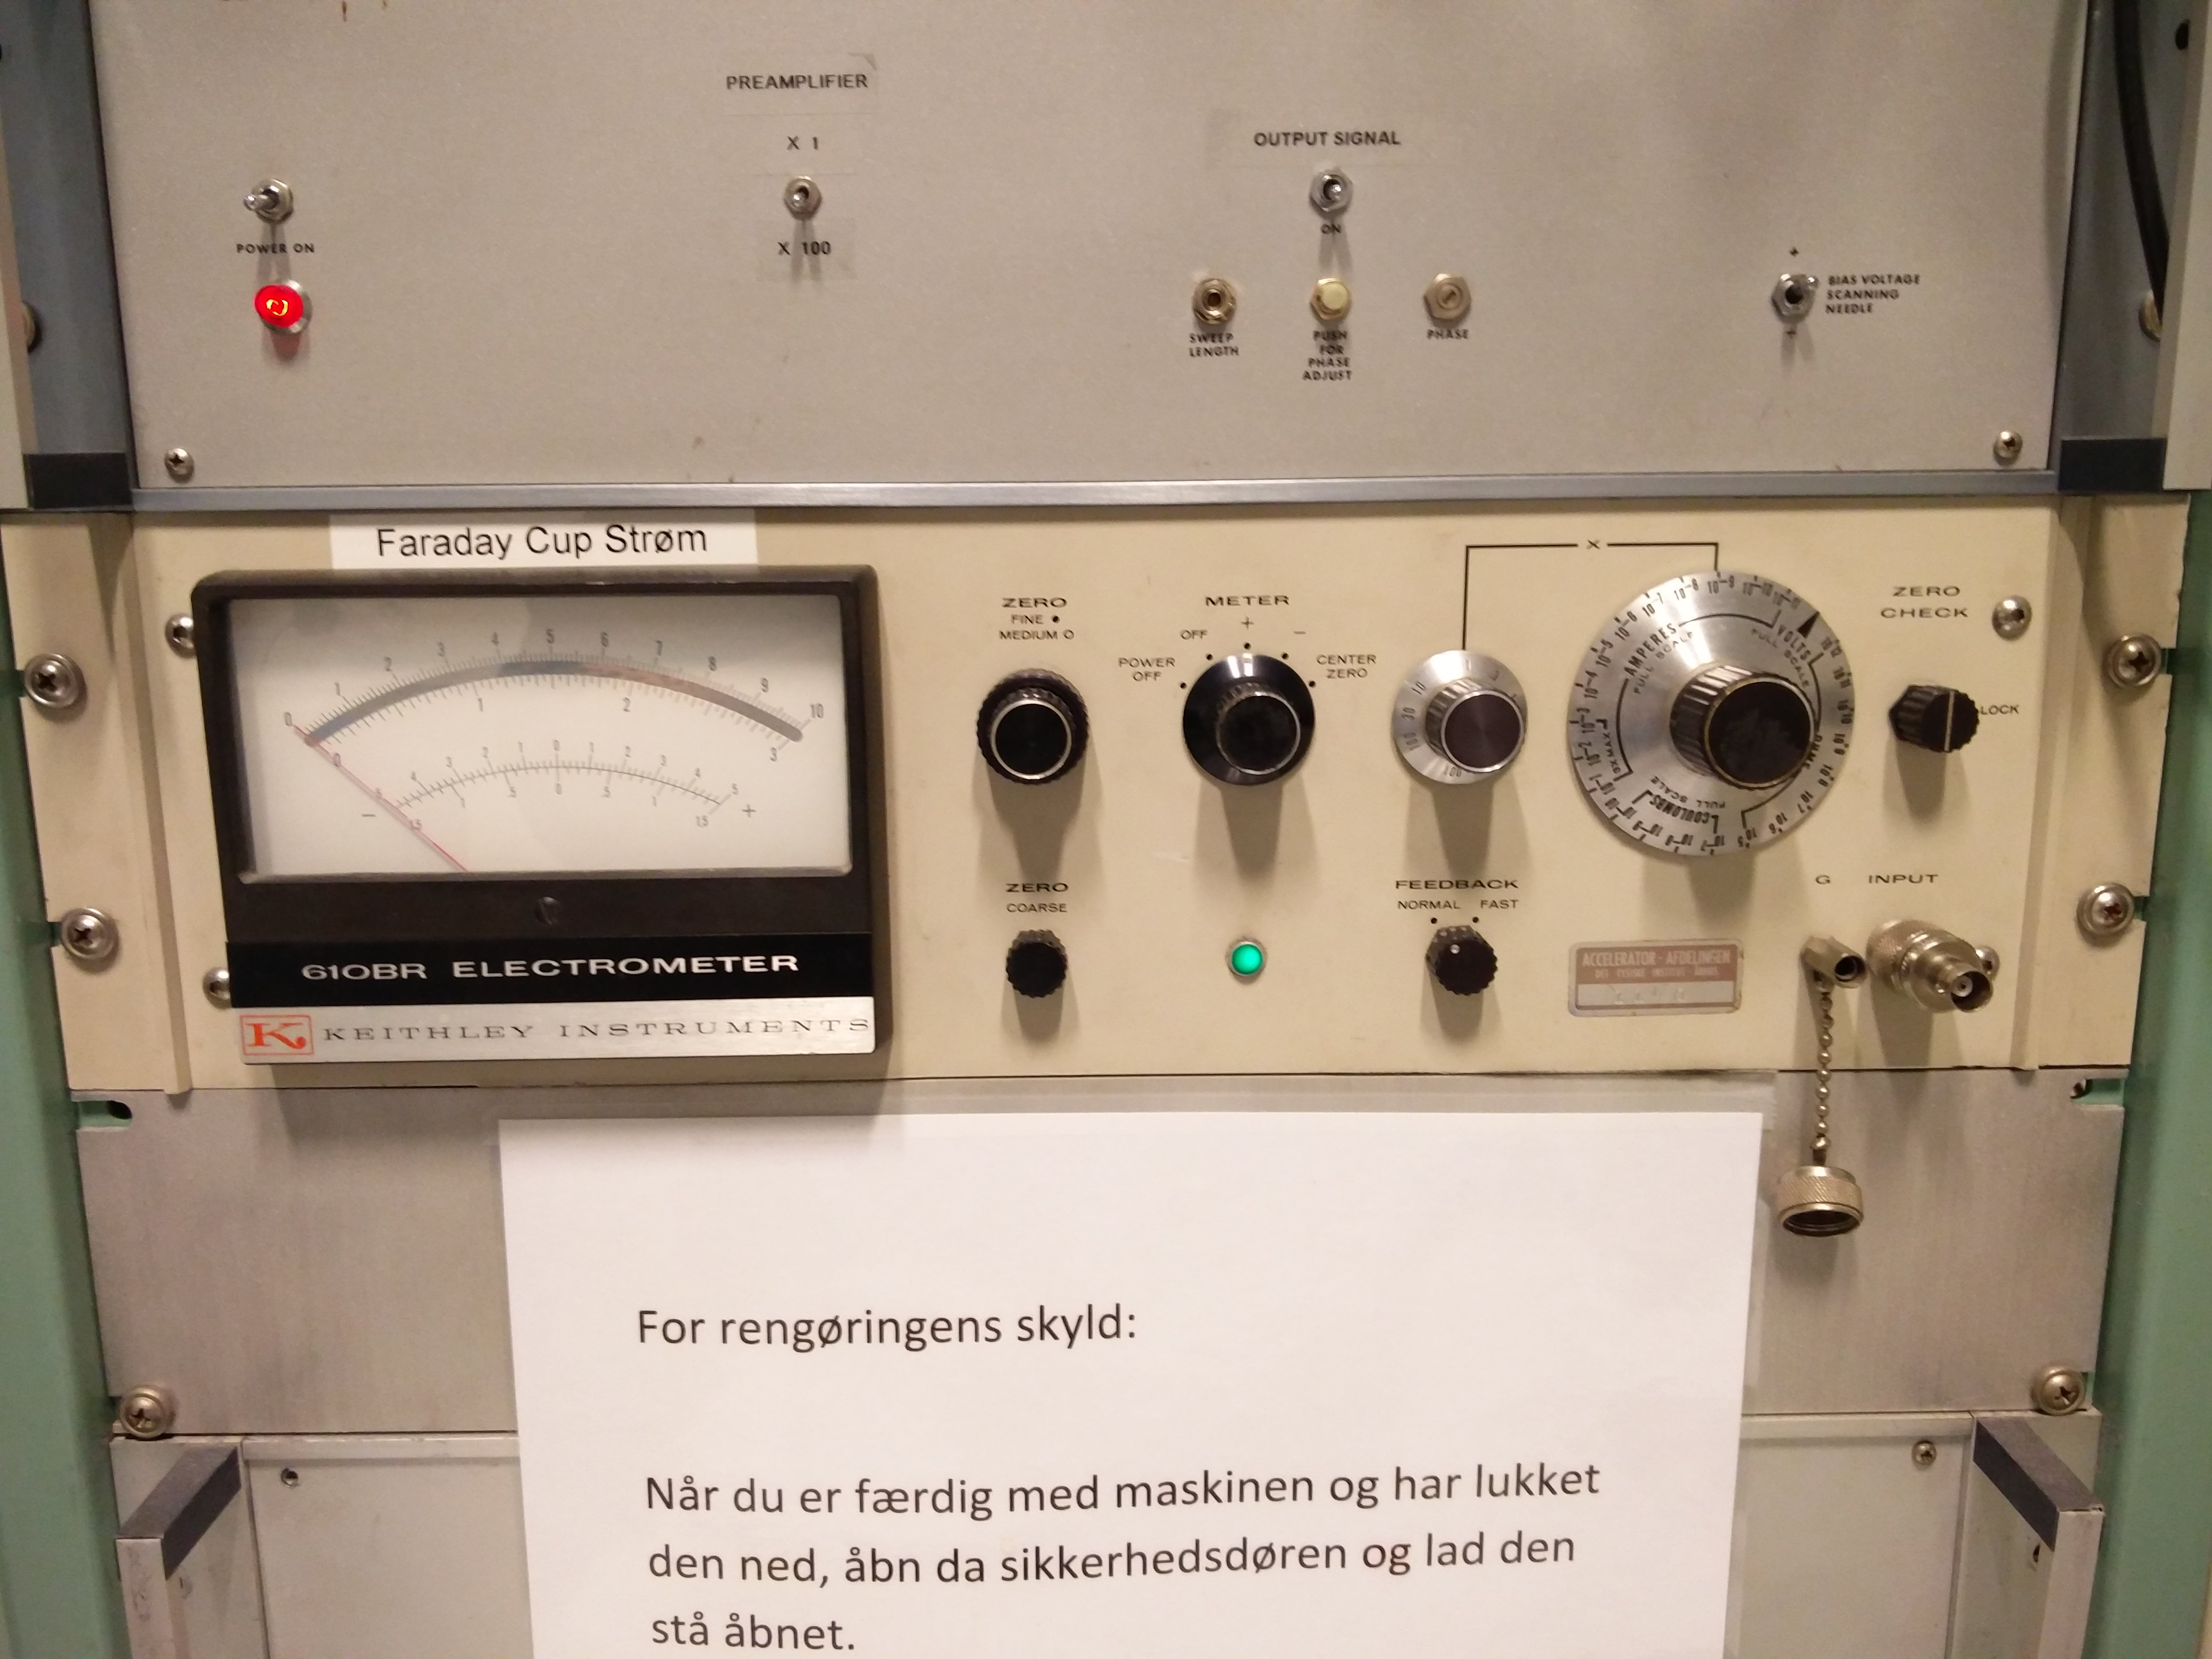
\includegraphics[trim={0, 35cm, 0, 30cm}, clip, width=0.99\columnwidth]{process4}
\caption{terminal voltage}
\label{fig_process4}
\end{figure}

When signal is good, set the voltage supply to ... 
\begin{figure}[h]
\centering
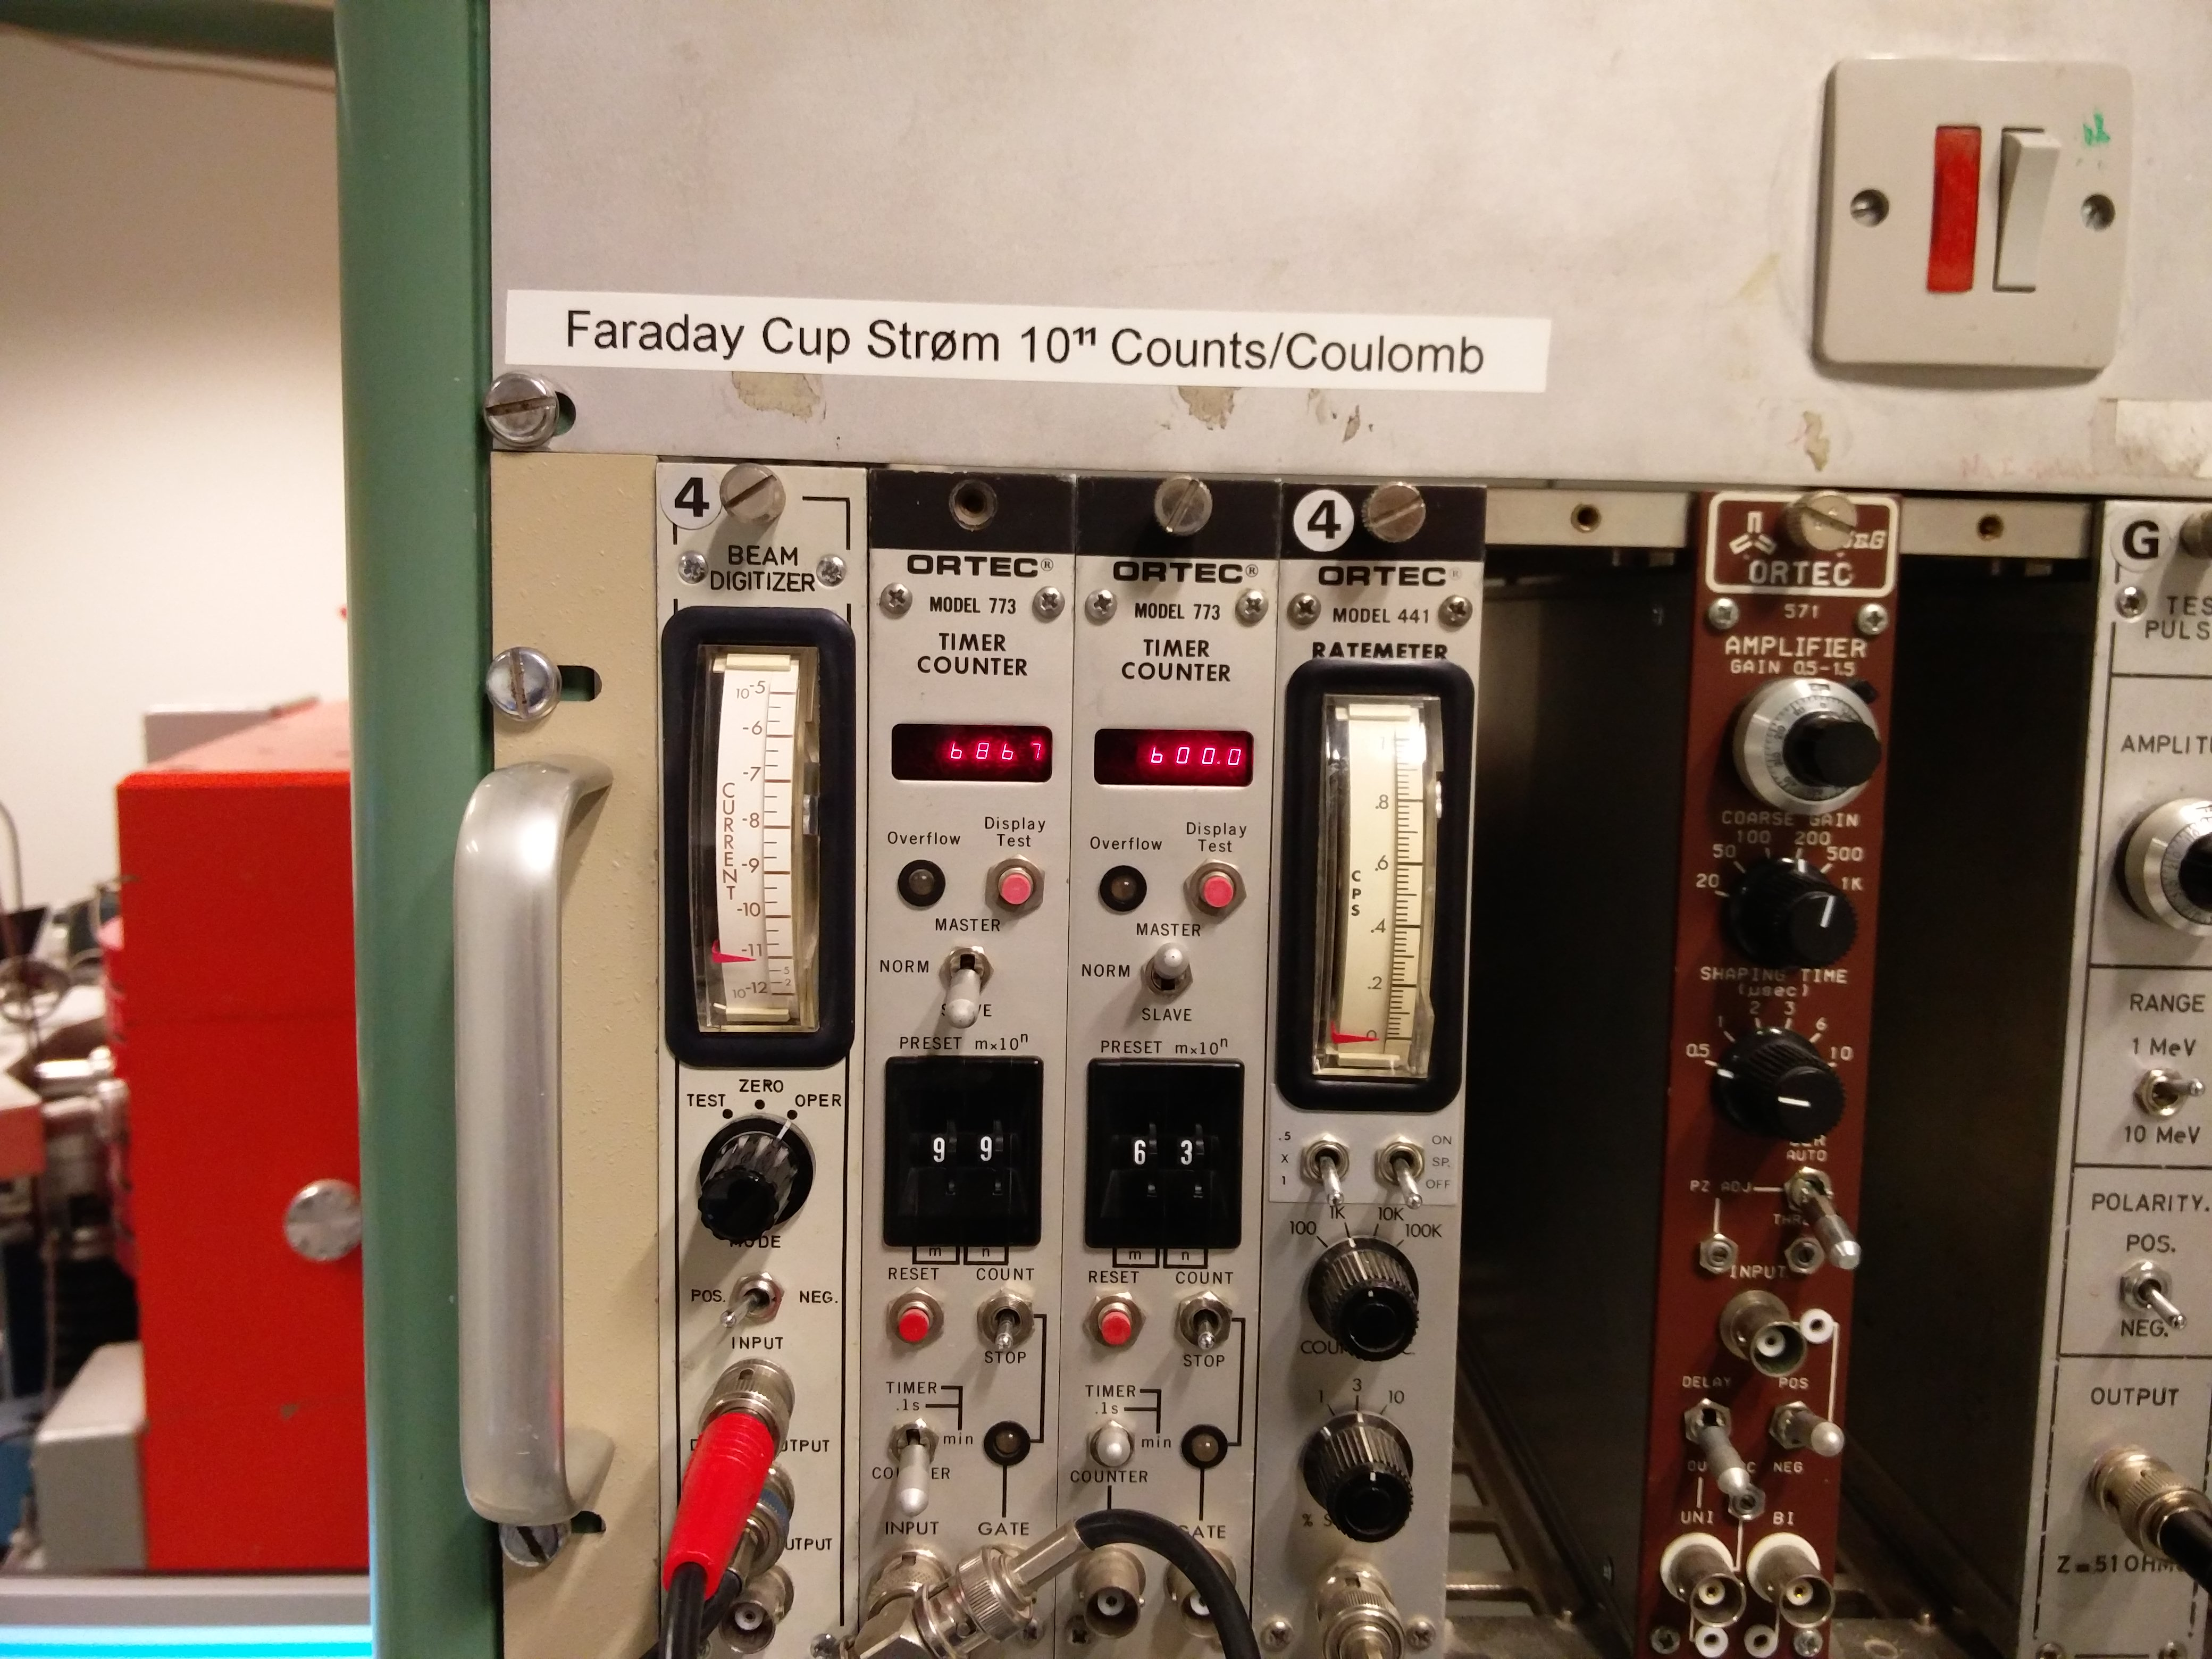
\includegraphics[trim={25cm, 0, 0, 15cm}, clip, width=0.99\columnwidth]{process5}
\caption{process5}
\label{fig_process5}
\end{figure}







